\documentclass{article}
\usepackage{amsmath}
\usepackage[margin=0.5in]{geometry}
\usepackage{amssymb,amscd,graphicx}
\usepackage{epsfig}
\usepackage{epstopdf}
\usepackage{hyperref}
\usepackage{color}
\usepackage[]{amsmath}
\usepackage{amsfonts}
\usepackage{amsthm}
\bibliographystyle{unsrt}
\usepackage{amssymb}
\usepackage{graphicx}
\usepackage{epsfig}  		% For postscript
%\usepackage{epic,eepic}       % For epic and eepic output from xfig
\renewcommand{\thesection}{}  % toc dispaly

\newcommand{\ds}{\displaystyle}
\newtheorem{thm}{Theorem}[section]
\newtheorem{prop}[thm]{Proposition}
\newtheorem{lem}[thm]{Lemma}
\newtheorem{cor}[thm]{Corollary}

\title{Pre-Calculus Notes}
\date
\Large
\begin{document}
\maketitle
\large

\tableofcontents


%%%%%%%%%%%%%%%%%%%%%%%%%
%%%%%%%%%%%%%%%%%%%%%%%%%
\section{Fun Stuff}
%%%%%%%%%%%%%%%%%%%%%%%%%
%%%%%%%%%%%%%%%%%%%%%%%%%

\begin{enumerate}
\item Feynman Method: \url{https://www.youtube.com/watch?v=FrNqSLPaZLc}
\item Bad math writing: \url{https://lionacademytutors.com/wp-content/uploads/2016/10/sat-math-section.jpg}
\item Google AI experiments: \url{https://experiments.withgoogle.com/ai}
\item Babylonian tablet: \url{https://www.maa.org/press/periodicals/convergence/the-best-known-old-babylonian-tablet}
\item Parabola in real world: \url{https://en.wikipedia.org/wiki/Parabola#Parabolas_in_the_physical_world}
\item Parabolic death ray: \url{https://www.youtube.com/watch?v=TtzRAjW6KO0}
\item Parabolic solar power: \url{https://www.youtube.com/watch?v=LMWIgwvbrcM}
\item Robots: \url{https://www.youtube.com/watch?v=mT3vfSQePcs}, riding bike, kicked dog, cheetah, backflip, box hockey stick
\item Cat or dog: \url{https://www.datasciencecentral.com/profiles/blogs/dogs-vs-cats-image-classification-with-deep-learning-using}
\item History of logarithm: \url{https://en.wikipedia.org/wiki/History_of_logarithms}
\item Log transformation: \url{https://en.wikipedia.org/wiki/Data_transformation_(statistics)}
\item Log plot and population: \url{https://www.google.com/publicdata/explore?ds=kf7tgg1uo9ude_&met_y=population&hl=en&dl=en#!ctype=l&strail=false&bcs=d&nselm=h&met_y=population&scale_y=lin&ind_y=false&rdim=country&idim=state:12000:06000:48000&ifdim=country&hl=en_US&dl=en&ind=false} 
\item Yelp and NLP: \url{https://github.com/skipgram/modern-nlp-in-python/blob/master/executable/Modern_NLP_in_Python.ipynb} \url{https://www.yelp.com/dataset/challenge}
\item Polynomials and splines: \url{https://www.youtube.com/watch?v=O0kyDKu8K-k}, Yoda / matlab, \url{https://www.google.com/search?q=pixar+animation+math+spline&espv=2&source=lnms&tbm=isch&sa=X&ved=0ahUKEwj474fQja7TAhUB3YMKHY8nBGYQ_AUIBigB&biw=1527&bih=873#tbm=isch&q=pixar+animation+mesh+spline}, \url{http://graphics.pixar.com/library/}
\item Polynomials and pi/taylor series: Matlab/machin \url{https://en.wikipedia.org/wiki/Chronology_of_computation_of_%CF%80} 
\url{https://en.wikipedia.org/wiki/Approximations_of_%CF%80#Machin-like_formula}
\url{https://en.wikipedia.org/wiki/William_Shanks}
\item Deepfake: face \url{https://www.youtube.com/watch?v=ohmajJTcpNk} \\
dancing \url{https://www.youtube.com/watch?v=PCBTZh41Ris}
\item Pi digit calculations: \url{https://en.wikipedia.org/wiki/Chronology_of_computation_of_%CF%80}, poor shanks...\url{https://en.wikipedia.org/wiki/William_Shanks}
\end{enumerate}


\section{Course Introduction}
%%%%%%%%%%%%%%%%%%%%%%%%%
%%%%%%%%%%%%%%%%%%%%%%%%%

\begin{enumerate}
%%%%%%%%%%%%%%%%%%%%%%%%%
\item Syllabus highlights
\begin{enumerate}
\item Grades: 
\begin{enumerate}
\item Know the expectation / what you are getting into.
\item 15perc A (excellent), 35perc B (good), 35perc C (satisfactory),10perc D (passing), some F (failing)
\item Expect lower grades than you are used to. I was a student once upon a time. I know what it's like to give some effort in a class and still get an A/B. Night before study, good enough? 
\item Turn in an exam / project. Did you do good work?
\item Many will start off doing good / satisfactory work. Improve to something more. C is not the worst thing in existence. These letters say nothing of your capability. 
\end{enumerate}
\item What does good mean? Good means good. Good job! Excellent means you showed some flair.
\item Expect: More work, more expectation on good writing.
\item Math is a challenging subject. Not a natural thing to think or write in. It takes work and practice to be better. My goal is to train you to be better and give you ideas of where it can go.
\item Fact that you are here shows you are smart and capable. Your goal should be to improve. 
\item Why do I do this? I do it out of respect for you. You are smart enough. I want you to gain something valuable here. I wouldn't do this job if I didn't think you were gaining something of value.
\end{enumerate}

%%%%%%%%%%%%%%%%%%%%%%%%%
\item Outline of this class
\begin{enumerate}
\item Most important idea: Function
\item How to reverse a function? Inverse function. Key example: Exponential and logarithms.
\item Trigonometry. 
\begin{enumerate}
\item Triangle, unit circle, graphs. 
\item Go deep with all connections. More than you could ever want.
\item Applications. Distance, waves, circular motion. Universal ideas here: sound, light, vibration, rotation of earth, atomic vibration, so much.
\end{enumerate}
\item Vectors and high dimensional space. Trigonometry is the foundation.
\end{enumerate}

%%%%%%%%%%%%%%%%%%%%%%%%%
\item Grand scheme of things. Where does this class sit inside all of mathematics.
%%%%%%%%%%%%%%%%%%%%%%%%%
\begin{enumerate}
\item Basics: Algebra, arithmetic.
\item First steps: Geometry, functions. (us now)
\item Calculus: Math of change / infinity.
\item Linear algebra: Math of vectors. Anything with finite representation. Invention of computers fueled this one. Gateway to real math / applications.
\item Applied math. Any application you want. Physics, finance, marketing, material science, CFD, sports. 
\item Abstract math. Create your own world of ideas. Number theory, analysis, algebra, topology, more. 
\end{enumerate}
\end{enumerate}

%%%%%%%%%%%%%%%%%%%%%%%%%%%%%%%%%%%%%%%%%%%%%%%%%%%%%%%%%%%%%%%%%%%%%%%%%%%%%%%%%%%%%%%%%%%%%%%%%%%%
%%%%%%%%%%%%%%%%%%%%%%%%%%%%%%%%%%%%%%%%%%%%%%%%%%%%%%%%%%%%%%%%%%%%%%%%%%%%%%%%%%%%%%%%%%%%%%%%%%%%
%%%%%%%%%%%%%%%%%%%%%%%%%%%%%%%%%%%%%%%%%%%%%%%%%%%%%%%%%%%%%%%%%%%%%%%%%%%%%%%%%%%%%%%%%%%%%%%%%%%%

\section{Chapter 4 Exponential and Logarithmic Functions}


%%%%%%%%%%%%%%%%%%%%%%%%%%%%%%%%%%%%%%%%%%%%%%%%%%%%%%%%%%%%%%%%%%%%%%%%%%%%%%%%%%%%%%%%%%%%%%%%%%%%
\subsection{4.0 Review: Functions and Inverse functions, Chapter 2 in text}
\begin{enumerate}

%%%%%%%%%%%%%%%%%%%%%%%%%%%%%%%%%%%%%%%%%%%%%%%%%%%%%%%%%%%%%%%%%%%%%%%%%%%%%%%%%%%%%%%%%%%%%%%%%%%%
\item Function (most important idea of this class)
\begin{enumerate}

%%%%%%%%%%%%%%%%%%%%%%%%%%%%%%%%%%%%%%%%%%%%%%%%%%%%%%%%%%%%%%%%%%%%%%%%%%%%%%%%%%%%%%%%%%%%%%%%%%%%
\item Basic idea of function
\begin{enumerate}
\item A function is a machine which takes an input and produces at most one output.
\item What is the domain / range of each? Key is that every input corresponds to at most one output.
\item Direction: input $\rightarrow$ output (card to bank account, bank account to card, are they the same association? Are they the same function?)
\item Restriction: When will things go wrong? One input to two output.
\item Domain: the collection of input
\item Range: the collection of output
\item Restricted domain: the range is automatically determined. Apply to one above example.
\end{enumerate}

%%%%%%%%%%%%%%%%%%%%%%%%%%%%%%%%%%%%%%%%%%%%%%%%%%%%%%%%%%%%%%%%%%%%%%%%%%%%%%%%%%%%%%%%%%%%%%%%%%%%
\item Mathematical setting
\begin{enumerate}
\item Numbers and variable (rather than any object)
\item Formal definition and percision of math language:  	A \underline{function} $f$ from set $X$ to $Y$, written $f:X\rightarrow Y$ is a relation which associates each element of $X$ with \emph{exactly} one element in $Y$. 
\item Notation: $y = f(x)= x^2, r = g(t)$, $f(-2)=4$
\item Domain: all possible $x$ 
\item Range: all possible $y$ (outputs)
\item Representations: Words (not common), formula, graph
\end{enumerate}

%%%%%%%%%%%%%%%%%%%%%%%%%%%%%%%%%%%%%%%%%%%%%%%%%%%%%%%%%%%%%%%%%%%%%%%%%%%%%%%%%%%%%%%%%%%%%%%%%%%%
\item {\bf Example:} Graph $f(x) = -2x+1$ and $g(x)=x^2-1$, list domain and range.

%%%%%%%%%%%%%%%%%%%%%%%%%%%%%%%%%%%%%%%%%%%%%%%%%%%%%%%%%%%%%%%%%%%%%%%%%%%%%%%%%%%%%%%%%%%%%%%%%%%%
\item Remarks
\begin{enumerate}
\item How to tell if equation is of a function? Graph and vertical line test. Are each a function of $x$? $y=x^2, x=y^2$.
\item To define a function, we need to
\begin{itemize}
\item Indicate the rule (formula)
\item State the domain (important)
\end{itemize}
\item If not specified, the domain is all the possible values
\begin{itemize}
\item Typical for even radicals, zero division
\item All real numbers $(-\infty, \infty)$
\end{itemize}
\end{enumerate}

%%%%%%%%%%%%%%%%%%%%%%%%%%%%%%%%%%%%%%%%%%%%%%%%%%%%%%%%%%%%%%%%%%%%%%%%%%%%%%%%%%%%%%%%%%%%%%%%%%%%
\item Interval notation
\begin{enumerate}
\item $(a,b)$: all the numbers between a and b
\item $($, $)$, exclude, $[$,$]$ include
\item $(a, \infty)$ all the numbers that are bigger than $a$
\item $(-\infty, b)$ all the numbers that are less than $b$
\end{enumerate}
\item {\bf Student Example:} Find the domain of each. Write in interval notation:
$$f(x) = 2- \sqrt{1+2x}, \quad g(x) = \sqrt{x-3}-\frac{1}{\sqrt{x+2}}, \quad h(x) = \frac{1}{2x^2+5x+2}$$

%%%%%%%%%%%%%%%%%%%%%%%%%%%%%%%%%%%%%%%%%%%%%%%%%%%%%%%%%%%%%%%%%%%%%%%%%%%%%%%%%%%%%%%%%%%%%%%%%%%%
\item Other function ideas
\begin{enumerate}
\item Major types of functions: Constants, lines, quadratics, polynomials, rationals, roots, exponential, log, trig, list goest on.
\item Symmetry: Even ($f(-x)=f(x)$ all $x$) / odd ($f(-x)=-f(x)$ all $x$) functions. 
\item Transformations: Shifts, stretches, reflections
\item Combinations: Sum, diff, prod, quotient, composition
\end{enumerate}
\end{enumerate}

%%%%%%%%%%%%%%%%%%%%%%%%%%%%%%%%%%%%%%%%%%%%%%%%%%%%%%%%%%%%%%%%%%%%%%%%%%%%%%%%%%%%%%%%%%%%%%%%%%%%
\item Inverse functions: Same association, the opposite direction. Reverse of a function.
\begin{enumerate}

%%%%%%%%%%%%%%%%%%%%%%%%%%%%%%%%%%%%%%%%%%%%%%%%%%%%%%%%%%%%%%%%%%%%%%%%%%%%%%%%%%%%%%%%%%%%%%%%%%%%
\item Big questions:
\begin{itemize}
\item How to tell if a function is invertible?
\item If $f$ is invertible, how to find it?
\item What is the relationship between a function and its inverse? (Domain/range, graph, etc)
\end{itemize}

%%%%%%%%%%%%%%%%%%%%%%%%%%%%%%%%%%%%%%%%%%%%%%%%%%%%%%%%%%%%%%%%%%%%%%%%%%%%%%%%%%%%%%%%%%%%%%%%%%%%
\item New mapping, given the output, find the input. Output $\rightarrow $ input. Once you know one direction, and you know it is invertible, you should know both directions.

%%%%%%%%%%%%%%%%%%%%%%%%%%%%%%%%%%%%%%%%%%%%%%%%%%%%%%%%%%%%%%%%%%%%%%%%%%%%%%%%%%%%%%%%%%%%%%%%%%%%
\item {\bf Student Examples:} $f(x) = -2x+1$ and $g(x)=x^2-1$. Given an output, which are invertible and why?
\begin{itemize}
\item One to one function: two distinct input cannot have the same output in original function $f$
\item Horizontal line test on graph
\end{itemize}

%%%%%%%%%%%%%%%%%%%%%%%%%%%%%%%%%%%%%%%%%%%%%%%%%%%%%%%%%%%%%%%%%%%%%%%%%%%%%%%%%%%%%%%%%%%%%%%%%%%%
\item Inverse function definition and notation: For $f$ one-to-one, the inverse of $f$, written $f^{-1}$ is the association which maps outputs of $f$ to corresponding inputs. That is,
\[
y=f(x) \quad \Longleftrightarrow f^{-1}(y)=x
\]

Note: There exists notational confusion.
$$
f^{-1} (x) \neq \frac{1}{f(x)}
$$

%%%%%%%%%%%%%%%%%%%%%%%%%%%%%%%%%%%%%%%%%%%%%%%%%%%%%%%%%%%%%%%%%%%%%%%%%%%%%%%%%%%%%%%%%%%%%%%%%%%%
\item How to find the inverse function $f^{-1}$ of a given function $f$?
\begin{itemize}
\item Check if it is one-to-one (HLT)
\item $y$ is known, so find $x$. Solve the equation $y=f(x)$ for $x$.
\item Write it in the standard way
\item Put the domain if necessary
\end{itemize}

%%%%%%%%%%%%%%%%%%%%%%%%%%%%%%%%%%%%%%%%%%%%%%%%%%%%%%%%%%%%%%%%%%%%%%%%%%%%%%%%%%%%%%%%%%%%%%%%%%%%
\item {\bf Example:} Find the inverse function of $f(x) = -2x+1$ (when is the output 1, -4, y?), graph $f$ and $f^{-1}$.
\begin{itemize}
\item Relation between graphs of $f$ and $f^{-1}$: reflection with respect to straight line $y=x$ (give examples)
\item Repeat with $g(x)=x^2-1$, restricted domain $x>0$. Why / where is the restriction needed?
\end{itemize}

%%%%%%%%%%%%%%%%%%%%%%%%%%%%%%%%%%%%%%%%%%%%%%%%%%%%%%%%%%%%%%%%%%%%%%%%%%%%%%%%%%%%%%%%%%%%%%%%%%%%
\item {\bf Student Example:}  A bit more challenging, find inverse of $f(x)  = \frac{x+2}{2x-1}$, list domain and range.
\item Fact
$$\text{range of $f$ = domain of $f^{-1}$}$$
$$\text{domain of $f$ = range of $f^{-1}$}$$

%%%%%%%%%%%%%%%%%%%%%%%%%%%%%%%%%%%%%%%%%%%%%%%%%%%%%%%%%%%%%%%%%%%%%%%%%%%%%%%%%%%%%%%%%%%%%%%%%%%%
\item Verifying inverse function of each other, refresh function composition: $(f\circ g)(x)=f(g(x))$.
$$
f(g(x)) = x \quad \text{ for any x in the domain of g}
$$
or
$$
g(f(x)) = x \quad \text{ for any x in the domain of f} 
$$
{\bf Example}: are they inverse function to each other: $f(x)  = \frac{x+2}{2x-1}, f^{-1}$ as above
\end{enumerate}
\end{enumerate}


%%%%%%%%%%%%%%%%%%%%%%%%%%%%%%%
%%%%%%%%%%%%%%%%%%%%%%%%%%%%%%%
\subsection{4.1 Exponential functions}
%%%%%%%%%%%%%%%%%%%%%%%%%%%%%%%
%%%%%%%%%%%%%%%%%%%%%%%%%%%%%%%

\begin{enumerate}

%%%%%%%%%%%%%%%%%%%%%%%%%%%%%%%
\item Motivation: Compound interest example. Invest 1000 dollars for a year at 5 percent interest compounded monthly. How much do you earn?
\begin{enumerate}
\item Quick example
\item General formula and explanation of each variable
\[
A = P\left(1+\frac{r}{n}\right)^{nt}
\]
\item Applied problem to find the amount given principal, compounding period, and rate. 
\end{enumerate}


%%%%%%%%%%%%%%%%%%%%%%%%%
\item Basic: Review laws of exponents! Refresher examples. \\
\begin{enumerate}
\item LoE: $a^0, a^1, a^ma^n, a^m/a^n, a^nb^n, (a/b)^n, a^{-n}$. 
\item {\bf Student Examples}: Simplify $\ds \frac{\sqrt[3]{ab}\cdot b^2}{a^3\cdot b^{1/2}}; (-27)^{2/3}(4)^{-5/2}; \left( \frac{2x^{2/3}}{y^{1/2}}\right)\left( \frac{3x^{-5/6}}{y^{1/3}}\right)$
\item What exponent means: $2^3, 2^{-1}, 2^{1/2}, 2^{-4/3}$, good for any rational number, $2^\pi, 2^i$ needs calculus, but we have faith..
\item Solving exponential equations
\begin{itemize}
\item {\bf Student Examples}: Solve for $x$: $\ds 2^{-x}=8; \quad 8^{2x}=\frac{1}{2^{2-x}}; \quad 3(3^x)+9(3^{-x})=28$ (rewrite as same base and hidden quadratic)
\end{itemize}
\end{enumerate}


%%%%%%%%%%%%%%%%%%%%%%%%%%%%%%%
\item Exponential function: $f(x) = a^x$
\begin{enumerate}
\item Definition: why $a>0$ and $a\neq1$
\item Graphs
\begin{itemize}
\item Concrete examples: $f(x)=2^x, 5^x, (1/3)^x=3^{-x}$
\item Domain and range
\item $a^0 = 1$ gives the same $y$-intercept
\item Increasing ($a>1$) / decreasing ($a<1$)
\item Shape: depends on the $a$
\item Horizontal Asymptote always at the $x$-axis
\item Note they are all one-to-one, so we should be able to invert them
\end{itemize}
\end{enumerate}

%%%%%%%%%%%%%%%%%%%%%%%%%%%%%%%
\item Reading exponential function
\begin{itemize}
\item Comparing base 
\item General format: $b\cdot a^x$
\item Identify graphs with points and shift
\end{itemize}

%%%%%%%%%%%%%%%%%%%%%%%%%%%%%%%
\item Intuition / examples:
\begin{itemize}
\item Exponential function grows fast (mark pen example)
\item Application: Student loan interest calculation, mortgage payment calculator. 
\end{itemize}
\end{enumerate}


%%%%%%%%%%%%%%%%%%%%%%%%%%%%%%%
%%%%%%%%%%%%%%%%%%%%%%%%%%%%%%%
\subsection{4.2 The Natural exponential functions}
%%%%%%%%%%%%%%%%%%%%%%%%%%%%%%%
%%%%%%%%%%%%%%%%%%%%%%%%%%%%%%%

\begin{enumerate}

%%%%%%%%%%%%%%%%%%%%%%%%%%%%%%%
\item Motivation: Need for a single, uniform base.
\begin{itemize}
\item Which one is bigger? ($3^4$ or $4^3$)
\item The idea of a uniform base(base is not unique $2^{3x}$, $4^x$)
\end{itemize}

%%%%%%%%%%%%%%%%%%%%%%%%%%%%%%%
\item The natural base $e$
\begin{enumerate}
\item Rather than lots of bases $a$, we would like a uniform base with nice properties (the natural exponential). Called natural since it shows up in interesting way (instantaneous, large populations and reproduction, many times, many things, life isn't always discrete).
\item Continuous compound interest:
\begin{itemize}
\item Invest \$1000 at 5\% per year.
$$
1000 + (0.05)1000 = 1050
$$
\item Same, twice a year, $\frac{5\%}{2}$ each time.
$$
1000 + (0.025)1000 + (0.025)(1000 + (0.025)1000)  = 
1000(1+0.05/2)^2 = 1050.625
$$
\item Quarterly, $\frac{5\%}{4}$ each time.
$$
1000(1+0.05/4)^4 = 1050.945
$$
\item Daily: 1051.267 (let students choose and guess here, per day second etc)
\item This seems to approach a limit / max.
\item Desmos: $(1+\frac{0.05}{n})^{n/0.05}$. 
\end{itemize}
\item Fact: modify above desmos, sort of growth rate 1.
$$
(1+\frac{1}{n})^n \rightarrow e,\quad\text{when } n\rightarrow \infty  
$$
where $e\approx 2.72$, Euler's number. Can show $e$ is irrational as important as $\pi$, if not more. Shows up in applications all the time. 
\item The natural exponential function $f$
$$
f(x) = e^x
$$
\end{enumerate}

%%%%%%%%%%%%%%%%%%%%%%%%%%%%%%%
\item Law of continuous growth formula
$$
q = q_0e^{rt}
$$
\begin{itemize}
\item $q_0$: initial quantity
\item r: the growth rate
\item t: time
\item e: natural base
\end{itemize}
\begin{enumerate}
\item Note:
\begin{enumerate}
\item $r>0$: growth rate
\item $r<0$: decay rate
\item $r$ is better in terms of identifying the increasing and decreasing rate, no longer have cases with the base
\item ``real" base: $e^r$
\end{enumerate}
\item Continuous compound interest.
\item When to apply: 
\begin{enumerate}
\item grows/decays proportional to its current value
\item continuously (instantaneously) changing 
\end{enumerate}
\item Uniform base: transform $y = ae^{kt}$ to $ab^t$ (still need logs to get here)
\end{enumerate}

%%%%%%%%%%%%%%%%%%%%%%%%%%%%%%%
\item Applications
\begin{itemize}
\item Continuous compound interest: $A=Pe^{rt}$
\item Population growth: $P=P_0e^{rt}$
\item Radioactive decay (half life)
\item Anything that grow/decays at a percentage
\item How to understand continuous (not all the time, but can happen any time)
\item \url{https://www.google.com/publicdata/explore?ds=kf7tgg1uo9ude_&met_y=population&idim=state:06000:48000&hl=en&dl=en#!ctype=l&strail=false&bcs=d&nselm=h&met_y=population&scale_y=lin&ind_y=false&rdim=country&idim=state:06000:48000:12000&ifdim=country&hl=en_US&dl=en&ind=false}
\end{itemize}
\end{enumerate}


%%%%%%%%%%%%%%%%%%%%%%%%%%%%%%%
%%%%%%%%%%%%%%%%%%%%%%%%%%%%%%%
\subsection{4.3-4.4 Logarithmic functions and log properties}


%%%%%%%%%%%%%%%%%%%%%%%%%
\begin{enumerate}
\item Basics
\begin{enumerate}
\item Finding growth rate involves finding an input corresponding to a known output. The inverse of exponential function (all one-to-one here).
\item Graph $f(x)=a^x$ for $a>1$ and $0<a<1$, automatically can draw $f^{-1}$. Name $f^{-1}(x)=\log_a(x)$.
\item Careful definition of logarithm (defined to be inverse).
$$
y = \log_ax \quad\text{if and only if}\quad x = a^y
$$
\item The log as a function:
\begin{enumerate}
\item Domain, range
\item Special point (1,0)
\item Special bases
\item Function composition of $a^x$ and $\log_a(x)$.
\begin{enumerate}
\item The logarithmic function with natural base: $\ln x$
\item The common logarithmic function: $y = \log x$.
\end{enumerate}
\end{enumerate}
\item {\bf Examples:} 
\begin{enumerate}
\item Compute $\log(1/100), \log_4(2), \log_5(1/5), \log^3(1), \log_8(4), \log_9(\sqrt{3})$ (easier to look at exponential form)
\item Solve for $x$: $\log_3(x+4)=\log_3(1-x)$ (one-to-one), $e^{2\ln(x)} = 9$ (inverses and domain restriction).  
\item Find the domain and range: $\ln(\ln x)$.
\end{enumerate}
\end{enumerate}

%%%%%%%%%%%%%%%%%%%%%%%%%
\item Applications: 
\begin{enumerate}
\item Originally for hand calculation because of log properties below. (Napier, slide rule, revolution of calculation)
\item Astronomical distance \url{https://en.wikipedia.org/wiki/Astronomical_system_of_units}
\item The Benford's law (first digit law) \url{https://en.wikipedia.org/wiki/Benford%27s_law}
\item Logarithmic transformation in data science: \url{https://en.wikipedia.org/wiki/Data_transformation_(statistics)}
\item Nature: \url{https://en.wikipedia.org/wiki/Logarithmic_spiral}
\item Solve exponential equation: $2{3x}=10$, $e^{2x}-3e^x+2=0$
\end{enumerate}

%%%%%%%%%%%%%%%%%%%%%%%%%
\item Log properties:
\begin{enumerate}
\item $\log_a (xy)$, $\log_a(x/y)$
\item $\log_a (x^p)$
\item $\log_a x = \frac{\log_b(x)}{\log_b(x)}$ change of base
\item $a^{\log_a x} = x,\quad\log_a a^x = x$ inverse relation
\item These are just the laws of exponents written in logarithmic form. Write $a^{s+t}, a^{st}, a^{-s}$ and draw parallels.
\begin{itemize}
\item Prod to sum: Let $\log_a(x)=s, \log_a(y)=t$, then $a^s=x, a^t = y$.
\item $xy = a^sa^t = a^{x+t}$, rewrite in log form
\item $\log_a(xy) = s+t = \log_a(x)+\log_a(y)$
\item Rest are same idea.
\end{itemize}
\item As mentioned before, make calculation easier (product to sum, power to product, etc).
\end{enumerate}

%%%%%%%%%%%%%%%%%%%%%%%%%
\item Typical problems
\begin{enumerate}
\item Express $\log_a \frac{x^3\sqrt{y}}{z^2}$ in terms of $\log x$, $\log y $, $\log z$
\begin{enumerate}
\item Split $\cdot$ and $/$
\item Bring down the power
\end{enumerate}
\item Express as one logarithm, opposite direction: $\ds \ln(x+1)-2\ln(x-1)+5\ln(x)$
\item Why are we doing this? Solving equations? Solve real life problem.
\begin{enumerate}
\item The population of La Crosse 50000 in 2000, 55000 in 2010, what will it be in 2020 assuming continuous growth? 
\item Which would you choose and why? Invest \$100 at 4\% or \$500 at 3\%? When do they equal? Depends on length of investment.
\item Google population of Florida, Cali, and Texas. Which is growing faster? Let them guess and explain why. Care about growth rate here, use log plot instead. Care about slope of this new line. Not a realistic fit globally though! Population of sad North Dakota
$$
y = Pe^{rt}, ~ \ln(y) = \ln(P)+rt, ~ z = c + rt
$$
\url{https://www.google.com/publicdata/directory} Possible project here, fit exponential, logistic growth, etc
\end{enumerate}
\end{enumerate}

%%%%%%%%%%%%%%%%%%%%%%%%%
\item Solving equations examples, these main ideas are all there is.
\begin{enumerate}
\item $8^{2x}(\frac{1}{4})^{x-2} = 4^{-x}$. Rewrite in same base.
\item $2^x = 3^{1-x}$, cannot rewrite in same base, use logarithm of any base. Many equivalent but different looking solutions. Nice bases to choose are 2,3.
\item $\log_3(-x) + \log_3(8-x) = 2$. Beware of domain changes. Always need to check solution. Only $x=-1$ works here.
\item Hidden quadratic: $e^{2x}-e^x-2 = 0$
\end{enumerate}

%%%%%%%%%%%%%%%%%%%%%%%%%
\item Transfer anything to base $e$: y = $2^x$
\begin{enumerate}
\item Connection between continuous and discrete cases
\item Everything is continuous
\item One formula but restrict your $x$ to be integer.

%%%%%%%%%%%%%%%%%%%%%%%%%
\item Groupwork handout, treat as take home quiz.
\begin{enumerate}
\item Tips: 
\item Remove the log
\item Check the domain
\end{enumerate}
\end{enumerate}
\end{enumerate}

%%%%%%%%%%%%%%%%%%%%%%%%%
%%%%%%%%%%%%%%%%%%%%%%%%%
\subsection{4.5 Exponential and logarithmic equations}
%%%%%%%%%%%%%%%%%%%%%%%%%
%%%%%%%%%%%%%%%%%%%%%%%%%

Group work take home quiz!

%%%%%%%%%%%%%%%%%%%%%%%%%
%%%%%%%%%%%%%%%%%%%%%%%%%
\subsection{4.6 Modeling with exponential functions}
Already discussed all this, just remind and formalize. New idea is that continuous growth assumes a population (or quantity) grows at a rate proportional to its size. Calculusness.
\begin{enumerate}
%%%%%%%%%%%%%%%%%%%%%%%%%
\item Population growth:
\begin{enumerate}
\item "Scheduled" growth: $P(t) = P_0 b^t$ (doubling time $a$ gives $P(t) = P_0 2^{t/a}$)
\item Continuous growth: $P(t) = P_0e^{rt}$ where $r$ is the relative growth rate (La Crosse example done)
\end{enumerate}

%%%%%%%%%%%%%%%%%%%%%%%%%
\item Radioactive decay of mass: $m(t) = m_0 e^{-rt}$.

%%%%%%%%%%%%%%%%%%%%%%%%%
\item Newton's law of cooling: $T(t) = T_s + T_0 e^{-kt}$.

%%%%%%%%%%%%%%%%%%%%%%%%%
\item Examples from text: 11 (population growth), 20 (radioactive decay),  27 (newton's law of cooling)


\end{enumerate}

%%%%%%%%%%%%%%%%%%%%%%%%%
%%%%%%%%%%%%%%%%%%%%%%%%%
\section{Chapter 5 Trigonometric functions: Right triangle approach}
\begin{itemize}
\item Does everybody know trigonometry? Definition discussion on day one, math of position, relate $xy$ to angle and magnitude
\item Trigonometry: greek words, trigonon(triangle) - metria (measurement)
\item Why is it useful? GPS, astronomy, surveying, music theory, acoustics, electronics, position and waves, interpret any signal as sine/cosine (Fourier series/transform).
\item Purpose of learning, physics, martial arts, example?
\end{itemize}

%%%%%%%%%%%%%%%%%%%%%%%%%
%%%%%%%%%%%%%%%%%%%%%%%%%
\subsection{5.1 Angle measures}
\begin{enumerate}  

%%%%%%%%%%%%%%%%%%%%%%%%%
\item Goal: Carefully define the idea of an angle (two units, applications too)

%%%%%%%%%%%%%%%%%%%%%%%%%
\item Definition of angle:  
\begin{enumerate}
\item Geometry: one vertex, two rays
\item Notation: $\angle \alpha$, $\angle AOB$
\item Initial side: OA, terminal side: OB
\item Unit: degree ($360^\circ$ for a whole circle. Why? Calendar, time, and nice divisions of 360.)
\item Angles bigger than 360 degree: draw some examples 
\begin{itemize}
\item Show it by rotating arrow
\item Coterminal angles
\item Positive (counter-clockwise), negative (clockwise)
\end{itemize}
\end{enumerate}
\item How to compare two angles? Put into standard position (put angle into coordinate systems).
\begin{enumerate}
\item How:
\begin{itemize}
\item Vertex: origin (0,0)
\item Initial side: positive x-axis
\item 4 quadrants
\end{itemize}	 
\item Positive/negative angle: give an example of angle AOB and BOA
\begin{itemize}
\item Positive: counterclockwise
\item Negative: clockwise
\end{itemize}
\item Notation: greek symbols without angle symbol
\item Draw a standard angle: give examples
\begin{itemize}
\item Terminal side
\item Rotating arrow
\end{itemize}
\item Which quadrant the terminal side lies in?
$$
\theta = 60^\circ,\quad \theta = -135^\circ,\quad \theta = 1200^\circ, \quad -700^{\circ}
$$
\item Adding and subtracting angle: transfer geometry into algebra
\item Coterminal angles $\alpha$, $\beta$: $\alpha-\beta$ is a multiple of $360^\circ$ (the senator of all angles)
\item All the coterminal angles with $\theta$: $\theta+2n\pi$, where n can be any integer (including negative)
\end{enumerate}

%%%%%%%%%%%%%%%%%%%%%%%%%
\item Angle terminology:
\begin{enumerate}
\item Right angle: $90^\circ$, perpendicular
\item Acute angle: $0<\theta<90^\circ$
\item Obtuse angle: $90^\circ<\theta<180^\circ$
\item Complementary angles $\alpha$, $\beta$: $\alpha+\beta = 90^\circ$
\item Supplementary angles $\alpha$, $\beta$: $\alpha+\beta = 180^\circ$
\item {\bf Example: } What's the complementary angle of $32^\circ$? Supplementary?
\end{enumerate}

%%%%%%%%%%%%%%%%%%%%%%%%%
\item Fractional angles:
\begin{enumerate}
\item Can use decimal representation: $90.5^{\circ}$.
\item Can also use degrees/minutes/seconds: $90^{\circ} 30' 0''$
\item Can convert easily, see text for more.
\[
31^{\circ} 41' 59'' = 31^{\circ} + \left(41 + \frac{59}{60}\right)' = \left(31+\frac{41}{60} + \frac{59}{360}\right)^{\circ} = 31.847...^{\circ}
\]
\end{enumerate}

%%%%%%%%%%%%%%%%%%%%%%%%%
\item Radian measure: 
\begin{enumerate}
\item When dealing with circles, new termonology for angle measure: radians.
\item Draw circle, center $C$, points $A,B$, radius $r$, central angle $\theta$, $\text{arc}(AB)$
\item One \emph{radian} is the measure of central angle $\theta$ after traveling one arc of length the radius. Draw!
\item How many radians per revolution? A bit more than 6.
\[
360^{\circ} = 2\pi \text{ radians } = 2\pi \text{(no label here, only label degrees)}
\]
\item Important angles to \emph{not memorize} $0^{\circ}, 30^{\circ}, 45^{\circ}, 60^{\circ}, 90^{\circ}, 180^{\circ}, 360^{\circ}$ convert to radians.
\item Let two people compete to draw angles in degree and radians
\item Relation between degree and radius
\begin{enumerate}
\item $360^\circ = 2\pi$ rad or $180^\circ = \pi$ rad
\item degree to radians: $\theta^{\circ} = \frac{\pi}{180}\theta \text{ radians}$
\item radians to degree: $\theta \text{ radians} = \frac{180}{\pi} \theta^{\circ}$\\
\item {\bf Example:} Convert each: $225^\circ$, $\frac{11\pi}{6}$, $\pi^\circ$, beware of labels!
\end{enumerate}
\end{enumerate}

%%%%%%%%%%%%%%%%%%%%%%%%%
\item Circumference and arc length formulas are easy in radians. Draw picture.
\begin{itemize}
\item A circle of radius $r$ has circumference $2\pi$.
\item The length of arc $s$ with central angle $\theta$ is $\theta r$.
\item Note, default angle unit is radians here! Degrees differ, especially with arc length. Need to convert.
\end{itemize}

%%%%%%%%%%%%%%%%%%%%%%%%%
\item The sector area formula. Again, no need to memorize. Instead, know the idea.
\begin{enumerate}
\item A circle of radius $r$ has area $\pi r^2$.
\item The area of sector $t$ with central angle $\theta$ is 
\[\pi r^2 \cdot \frac{\theta}{2\pi} = \frac{1}{2}\theta r^2\]
\item {\bf Example:} which one you would buy? A half 9" pizza or a slice from a 20" pizza
\end{enumerate}

%%%%%%%%%%%%%%%%%%%%%%%%%
\item Angular and linear speed, allow change of these over time.
\begin{enumerate}
\item If angle changes, point $P$ moves around the circle. These are connected, how?
\[
s = \theta r \quad\Rightarrow\quad \frac{s}{t} = r \left(\frac{\theta}{t}\right), \quad (\text{linear speed = $r \cdot$ (angular speed)})
\]
\item A clock with a 3ft long minute hand and an 2ft long hour hand. What are the angular/linear speed for both hands?
\item Why do we care? Wind generators, clock gears, bike gears, body joint movement, astronomy etc
\item RMP: 55pmh on 28 inch diameter tires. What is the angular speed in RPMs? Unit conversions!
\[
\frac{s}{t} = 55 \frac{mi}{h} = 55 \frac{mi}{h} \frac{1 hr}{60 min} \frac{5280 ft}{1 mi} \frac{12 in}{1 ft} 
= \frac{55\cdot 5280 \cdot 12}{60} \frac{in}{min} = 14 \left(\text{angular speed in} \frac{rads}{min}\right)
\]
\[
\text{angular speed} = \frac{55\cdot 5280 \cdot 12}{60 \cdot 14} \frac{rads}{min} = \frac{55\cdot 5280 \cdot 12}{60 \cdot 14} \frac{rads}{min} \frac{1 rev}{2\pi rads} =  660.265 RMP
\]
\item Bigger tire = gas saver?
\item 7000 RMP, max of 120 mpg, what is the tire diameter?
\end{enumerate}
\end{enumerate}


%%%%%%%%%%%%%%%%%%%%%%%%%
%%%%%%%%%%%%%%%%%%%%%%%%%
\subsection{5.2 Trigonometry of right triangles}
\begin{enumerate}

%%%%%%%%%%%%%%%%%%%%%%%%%
\item We have angles, now let's return to triangles. How are the 3 sides related to an interior angle? (draw a right triangle, identify the adjacent, opposite and hypotenuse sides)
\begin{enumerate}
\item Definition of all the six trig functions
\begin{enumerate}
\item {\bf Example:} If $\csc(\theta) = \frac{\sqrt{13}}{3}$ for $\theta$ acute, find $\tan(\theta)$. Hint by drawing triangle, need hypotenuse.
\item Pythagorean Theorem is needed (write down, why? picture proof, amazing)
\end{enumerate}
\item Trigonometric values have nothing to do with the size of the triangle, show similar triangles
\item These 6 are functions of $\theta$ where 
\begin{enumerate}
\item Input is naturally in radians (reason to come)
\item Domain main 3 (for now acute angles, but will push ahead later)
\item Range main 3 (for acute angles)
\item Important interval: $0<\sin (\theta)<1$, $0<\cos (\theta)< 1$
\item Random triangles to motivate above
\end{enumerate}
\end{enumerate}

%%%%%%%%%%%%%%%%%%%%%%%%%
\item Identities you need to know
\begin{enumerate}
\item Pythagorean theorem
\item Reciprocal identities: $\sin (\theta) = 1/\csc(\theta)$... etc (6 in total)
\item The tangent and cotangent identities
$$
\tan(\theta) = \frac{\sin (\theta)}{\cos (\theta)},\quad\cot(\theta) = \frac{\cos(\theta)}{\sin(\theta)}
$$
\item The Pythagorean identities (super important), show first via general triangle then rest come from first by division.
$$
\sin^2(\theta)+\cos^2(\theta) = 1,\quad \tan^2(\theta)+1 = \sec^2(\theta),\quad \cot^2(\theta)+1 = \csc^2(\theta)
$$
\end{enumerate}

%%%%%%%%%%%%%%%%%%%%%%%%%
\item How to use the identities
\begin{enumerate}
\item Special right triangles $30^\circ$/$60^\circ$ (comes from equilateral triangle), $45^\circ$ (comes from two sides the same). If other, use a calculator....for now.
\item Nice Pythagorean triples (3,4,5),(5,12,13), (7, 24, 25), etc
\item Knowing one trig function, can find all the trig values for acute $\theta$, more angles later.
\item Solving right triangles (note that if you just have the trig info, the triangle is not unique, similar triangles)
\begin{itemize}
\item {\bf Example:} $b = 6$, $\sin(\theta) = \frac{3}{5}$, find $a$, $c$
\item {\bf Example:} $\tan(\theta) = \sqrt{3}/3$, $c = 5$, find everything else including complimentary angle. 
\item Similar triangles show up.
\end{itemize}

%%%%%%%%%%%%%%%%%%%%%%%%%
\item Word problem fun: Section 5.2, 61. Highlight the overall strategy without being given a picture. Focus is turning description into math / triangles.

\end{enumerate}
\end{enumerate}


%%%%%%%%%%%%%%%%%%%%%%%%%
%%%%%%%%%%%%%%%%%%%%%%%%%
\subsection{5.3 Trigonometric functions of angles}

%%%%%%%%%%%%%%%%%%%%%%%%%
\begin{enumerate}

%%%%%%%%%%%%%%%%%%%%%%%%%
\item We have angles bigger than acute angles. How to trig those? 
\begin{enumerate}
\item Draw $\theta$ be a angle in standard position and $P(x,y)$ be any point on the terminal side of $\theta$ in the first quadrant.
\item $\theta = 0^{\circ}$, $\theta = 90^{\circ}$, move the terminal side approaching the $x$-axis, $y$-axis, what do each approach? So our ration definitions still make sense for these flattened triangles!
\item For other quadrants, (draw for quadrant 2), need to be ok with generalizing to triangles with negative sides. Always draw \emph{reference triangle} with acute \emph{reference angle} to keep us sane.
\begin{itemize}
\item Examples: Compute each $\cos(240 degrees), \csc(495 degrees), \cot(16\pi/3), \sec(-13\pi/4)$
\end{itemize}
\item Complete trig function definitions: For angle $\theta$ in standard position and $(x,y)$ a point on its terminal side, if the hypotenuse is $r = \sqrt{x^2+y^2}$, then 
$$
\sin \theta = \frac{y}{r}, \quad \text{etc, draw picture}
$$
\begin{enumerate}
\item Domain and range of each:
\item Trigonometric values can be negative, which quadrants does each occur (draw 4 quadrants, have them fill in signs of six trig fcns), also list where undefined on $xy$ axis.
\end{enumerate}
\end{enumerate}

%%%%%%%%%%%%%%%%%%%%%%%%%
\item {\bf Examples:}
\begin{enumerate}
\item If $P(3,-4)$ is on the terminal side of $\theta$, find all the trig values of $\theta$. Find the quadrant containing $\theta $. Draw a reference triangle with reference angle $\theta_R$ to make discussion easier.
\item If $\sin \theta = 3/5$, find $\tan(\theta)$? 2 cases here, note the nice symmetry (reminds of even functions, hint to later.). If $\frac{\pi}{2}\leq \theta\leq \pi$, find all the trig values of $\theta$. Again draw reference triangle.
\end{enumerate}

%%%%%%%%%%%%%%%%%%%%%%%%%
\item Formula for area of a triangle: $A=\frac{1}{2}ab\sin(\theta)$ where $\theta$ is between $a$ and $b$. Draw a picture. Why is this true?


%%%%%%%%%%%%%%%%%%%%%%%%%
\item {\bf Example:} Excel spreadsheet challenge! Give them sine/cosine values for 0,1,2,...,,45 degrees. Randomly generate 6ish angles between -1000 and 1000 degrees, one for each trig function. How many can they get in 10 minutes?
\begin{itemize}
\item Note: Need cofunction ideas here. Give example with $\cos(61)$ first.
\end{itemize}

\end{enumerate}

%%%%%%%%%%%%%%%%%%%%%%%%%%%%%%%%%%%%%%%%%%%%%%%%%%%%%%%%%%%%%%%%%%%%%%%%%%%
%%%%%%%%%%%%%%%%%%%%%%%%%%%%%%%%%%%%%%%%%%%%%%%%%%%%%%%%%%%%%%%%%%%%%%%%%%%
\subsection{5.4 Inverse Trigonometric Functions and Right Triangles}
%%%%%%%%%%%%%%%%%%%%%%%%%%%%%%%%%%%%%%%%%%%%%%%%%%%%%%%%%%%%%%%%%%%%%%%%%%%
%%%%%%%%%%%%%%%%%%%%%%%%%%%%%%%%%%%%%%%%%%%%%%%%%%%%%%%%%%%%%%%%%%%%%%%%%%%

\begin{enumerate}
%%%%%%%%%%%%%%%%%%%%%%%%%
\item Example: Find ALL $\theta$ such that $\sin(\theta) = -\frac{1}{2}$. Stumble across symmetry and periodicity.

%%%%%%%%%%%%%%%%%%%%%%%%%
\item Fill out all 4 quadrants with the nice angles (0, 30, 45, 60, 90) and reflections of these.

%%%%%%%%%%%%%%%%%%%%%%%%%
\item Motivation: $\sin(x)=\frac{1}{3}$
\begin{enumerate}
\item Our calculator can solve equations like this. What is really going on?
\item Draw the unit circle and show sticking point. Not a nice angle. 
\end{enumerate}

%%%%%%%%%%%%%%%%%%%%%%%%%
\item Inverse function review: 
\begin{enumerate}
\item Inverse relationship, expression, domain and range.
\item Are all functions invertible? Need one-to-one. Reversing may not be unique.
\item Even though $f(x)=x^2$ is not invertible, we can still solve equations like $x^2=25$. Key is domain restriction to make invertible, then use special features of the function. This is key idea for inverse trig, and we already do this to solve equations.
\end{enumerate}

%%%%%%%%%%%%%%%%%%%%%%%%%
\item Inverse sine:
\begin{enumerate}
\item Draw unit circle to show not one-to-one. Already know this because of symmetry / periodicity.
\item How to restrict the domain so take on each output in $[-1,1]$ only once? Let them decide. Many ways, which is best?
\item Restricted sine: $y=\sin(x), \quad -\frac{\pi}{2}\leq x \leq \frac{\pi}{2}$. All outputs for sine $[-1,1]$ are realized only once.
\item Draw unit circle for restricted sine.
\item Def: $y = \sin(x) \Leftrightarrow \arcsin(y)=x$
\item Notation: $\arcsin(x)=\sin^{-1}(x)$, but we like $\arcsin$ to avoid exponent confusion.
\item Domain restriction is confusing: $y = \arcsin(x)$ is the inverse function of RESTRICTED sine.
\end{enumerate}

%%%%%%%%%%%%%%%%%%%%%%%%%
\item {\bf Example:} Solve $\sin(x) = \frac{1}{3}$ via $\arcsin$ on $[0,\pi/2], [0, \pi],$ everywhere.
\begin{enumerate}
\item Draw unit circle, $x=\arcsin(1/3)$ gives solution on $[-\frac{\pi}{2},\frac{\pi}{2}]$.
\item Get the second solution on the unit circle, then periodicity.
\item Issue: We can write down the solution, but what is $\arcsin(1/3)$?
\item This issue is analogous to logarithms. $2^x=10$ gives $x=\log_2(10)$ which is not nice. Calculus gives logarithnmic tables and slide rules for this. Inverse trig has similar story.
\item Have them repeat for $\cos(x) = \frac{1}{3}$.
\end{enumerate}

%%%%%%%%%%%%%%%%%%%%%%%%%
\item What about the rest? Have them fill in a table.
\begin{enumerate}
\item $\sin, \cos, \tan$
\item Invertible? Yes or no.
\item Restricted domain
\item Range
\item Part of unit circle
\item What about the buddy functions? ($\sec, \csc, \cot$)
\end{enumerate}

%%%%%%%%%%%%%%%%%%%%%%%%%
\item Inverse relations:
\begin{enumerate}
\item $\sin(\arcsin(y)) = y, \quad -1\leq y \leq 1$
\item $\arcsin(\sin(\theta)) = \theta, \quad -\frac{\pi}{2}\leq \theta \leq \frac{\pi}{2}$
\item Note the domain restriction subtlety.
\item What about $\cos,\tan$?
\item {\bf Examples:}
\begin{enumerate}
\item $\sin(\arcsin(-1/2)) = -1/2$
\item $\arcsin(\sin(\frac{5\pi}{3})) = $? Cannot use the identity since not in restricted domain. Subtract $2\pi$ via periodicity and life is grand.
\end{enumerate}
\end{enumerate}

%%%%%%%%%%%%%%%%%%%%%%%%%
\item {\bf Student Examples :}
\begin{enumerate}
\item $\arccos(-1/2)$ (Call angle $\theta$, then travel through the inverse relation. Unit circle and restricted domain and reference triangles.)
\item $\tan(\arctan(12))$
\item $\arcsin(\cos(\pi/6))$
\item $\arcsin(\sin(5\pi/6))$
\item $\cos(\text{arcsec}(2))$
\item $\sin(\arccos(3/5))$
\end{enumerate}

%%%%%%%%%%%%%%%%%%%%%%%%%
\item Verifying trigonometric identities
\begin{enumerate}
\item $\cos(\arcsin(x)) = \sqrt{1-x^2}$ (Weird? Or not?)
\end{enumerate}
\end{enumerate}


%%%%%%%%%%%%%%%%%%%%%%%%%%%%%%%%%%%%%%%%%%%%%%%%%%%%%%%%%%%%%%%%%%%%%%%%%%%
%%%%%%%%%%%%%%%%%%%%%%%%%%%%%%%%%%%%%%%%%%%%%%%%%%%%%%%%%%%%%%%%%%%%%%%%%%%
\subsection{5.5 Law of Sines}
%%%%%%%%%%%%%%%%%%%%%%%%%%%%%%%%%%%%%%%%%%%%%%%%%%%%%%%%%%%%%%%%%%%%%%%%%%%
%%%%%%%%%%%%%%%%%%%%%%%%%%%%%%%%%%%%%%%%%%%%%%%%%%%%%%%%%%%%%%%%%%%%%%%%%%%

\begin{enumerate}
%%%%%%%%%%%%%%%%%%%%%%%%%
\item The primary goal of the next 2 sections is to extend trigonomety beyond right triangles. 
\begin{enumerate}
\item An oblique triangle is a triangle with no right angles.
\item Can still make use of right triangle trig. Use top picture.
\begin{center}
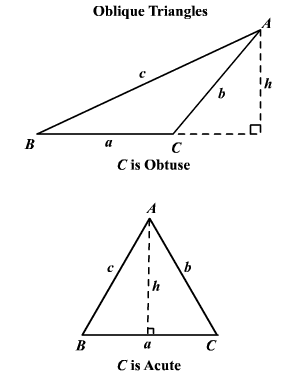
\includegraphics[width=0.3\textwidth]{sines.png}
\end{center}
\item How are $A,B,C,a,b,c$ related? Create a right triangle.
\[
\sin(B) = \frac{h}{c}, \quad \sin(C) = \cos(\frac{\pi}{2}-C) = \frac{h}{b} 
\]
\[
h = c\sin(B) = b\sin(C) \quad \Rightarrow \quad \frac{\sin(B)}{b} = \frac{\sin(C)}{c}
\]
\end{enumerate}

%%%%%%%%%%%%%%%%%%%%%%%%%
\item The law of sines:
$$
\frac{\sin (A)}{a} = \frac{\sin(B)}{b} = \frac{\sin(C)}{c}
$$
\begin{enumerate}
\item Note, this is actually 3 equations.
$$
\frac{\sin(A)}{a} = \frac{\sin(B)}{b}, \quad \frac{\sin(A)}{a} = = \frac{\sin(C)}{c}, \quad \frac{\sin(B)}{b} = = \frac{\sin(C)}{c}
$$
\item Also, geometry gives a fourth: $A+B+C=\pi$.
\end{enumerate}

%%%%%%%%%%%%%%%%%%%%%%%%%
\item How much information ($a,b,c,A,B,C$) is needed to solve a general triangle?
\begin{enumerate}
\item For right triangles, we need: (a) 2 sides or (b) 1 angle/1 side. Why does 2 angles not work? Note, we actually given 3 things here (right angle).
\item For general oblique triangle, need 3 things (not all angles). What are all the cases? Write all out. Which can we use law of sines on?
\begin{itemize}
\item Case 1: ASA/AAS (LoSines)
\item Case 2: SSA (LoSines)
\item Case 3: SAS (LoCosines) Why can't we handle these?
\item Case 4: SSS (LoCosines) Why can't we handle these?
\item Case 5: AAA (hopeless for uniqueness by similar triangles)
\end{itemize}
\end{enumerate}

%%%%%%%%%%%%%%%%%%%%%%%%%
\item {\bf Examples:}
\begin{enumerate}
\item Solve the triangle with $A=40^\circ, B=60^\circ, a=4$. What case is this? ASA. Can we use LoSines? Yes.
\begin{enumerate}
\item $C = 80^{\circ}, b = \frac{4\sin(60}{\sin(40)}, c = \frac{4\sin(80)}{\sin(40)}$
\end{enumerate}
\item Solve the triangle with $A=35^\circ, a=6, b=8$. What case is this? SSA. Can we use LoSines? Yes, but...difficulty.
\begin{enumerate}
\item Find $B$ first. $\sin(B) = \frac{4\sin(35)}{3}\approx 0.76$. 2 solutions here! Does this make sense? Yes, swing the leg and see two possible triangles.
\item Case 1: $B<90$, $C=95.1, c = \frac{6\sin(95.1)}{\sin(35)}$
\item Case 2: $B>90$, $C=14.9, c = \frac{6\sin(14.9)}{\sin(35)}$
\item This is why SSA is in its own class. Does it always yeild 2 solutions? Think leg swinging....could be one unique solution ($\sin(B)=1$, right triangle) or no solution ($\sin(B)>1$, too short). 
\end{enumerate}
\end{enumerate}

%%%%%%%%%%%%%%%%%%%%%%%%%
\item {\bf Examples:} The real purpose? Applications. More in take home quiz.
\begin{enumerate}
\item pg 481, 36,
\item pg 481, 37, \quad $h=175$ feet
\item pg 481, 40, \quad $??$ degrees.

%%%%%%%%%%%%%%%%%%%%%%%%%
\item Skip above applied problems, give take home quiz instead after covering Law of Cosines.

\end{enumerate}
\end{enumerate}



%%%%%%%%%%%%%%%%%%%%%%%%%%%%%%%%%%%%%%%%%%%%%%%%%%%%%%%%%%%%%%%%%%%%%%%%%%%
%%%%%%%%%%%%%%%%%%%%%%%%%%%%%%%%%%%%%%%%%%%%%%%%%%%%%%%%%%%%%%%%%%%%%%%%%%%
\subsection{5.6 The law of cosines}
%%%%%%%%%%%%%%%%%%%%%%%%%%%%%%%%%%%%%%%%%%%%%%%%%%%%%%%%%%%%%%%%%%%%%%%%%%%
%%%%%%%%%%%%%%%%%%%%%%%%%%%%%%%%%%%%%%%%%%%%%%%%%%%%%%%%%%%%%%%%%%%%%%%%%%%

\begin{enumerate}

%%%%%%%%%%%%%%%%%%%%%%%%%
\item Two remaining cases leftover from Law of Sines:
\begin{enumerate}
\item SAS
\item SSS
\end{enumerate}

%%%%%%%%%%%%%%%%%%%%%%%%%
\item The Law of Cosines (generalized Pythagorean theorem, all one formula by symmetry)
\begin{enumerate}
\item $a^2 = b^2+c^2-2bc\cos(A)$
\item $b^2 = a^2+c^2-2ac\cos(B)$
\item $c^2 = b^2+a^2-2ab\cos(C)$
\end{enumerate}
Note: No ambiguous case possible for Law of Cosines.

%%%%%%%%%%%%%%%%%%%%%%%%%
\item {\bf Example}: Solve the triangle with $c=45^{\circ}, A=15, B=10$. What case? Why can we not use Law of Sines at first? Use LoS as a second step and take car of multiple possibilities despite there being only a single solution.

%%%%%%%%%%%%%%%%%%%%%%%%%
\item Heron's formula
$$
A = \sqrt{s(s-a)(s-b)(s-c)}
$$
where $s = \frac{1}{2}(a+b+c)$
\begin{enumerate}
\item Demonstrate on 3,4,5 right triangle and compare to usual area formula.
\item Project 5
\end{enumerate}
\end{enumerate}


%%%%%%%%%%%%%%%%%%%%%%%%%
%%%%%%%%%%%%%%%%%%%%%%%%%
\section{Chapter 6: Trig functions and the unit circle approach}
%%%%%%%%%%%%%%%%%%%%%%%%%
%%%%%%%%%%%%%%%%%%%%%%%%%

Chapter 5 is about geometry / triangles. Here we extend trig to further ideas (general functions, rotations, etc).

%%%%%%%%%%%%%%%%%%%%%%%%%
%%%%%%%%%%%%%%%%%%%%%%%%%
\subsection{6.1 The unit circle}
%%%%%%%%%%%%%%%%%%%%%%%%%
%%%%%%%%%%%%%%%%%%%%%%%%%

\begin{enumerate}

%%%%%%%%%%%%%%%%%%%%%%%%%
\item Noted last time that the size of the triangle (similar triangles) yields the same trig values. Let's fix $r=1$ to make life nicer. Draw in $xy$-plane, this draws the unit circle as $\theta$ varies.
\begin{enumerate}
\item Suppose $\theta$ is a real number and $P(x,y)$ is the point on the unit circle that corresponds to $\theta$, then
$$
\sin(\theta) = y, \quad \cos(\theta) = x, \dots
$$ 
Note the book uses $t$ as a parameter for time.
\item Note $(x,y)$ here, new coordinate system (polar coordinates). More later.
\item What is the equation of a circle? $x^2+y^2=1$. Why? Distance formula / Pythagorean theorem, all the same. Note again $\sin^2(x)+\cos^2(x)=1$.
\end{enumerate}

%%%%%%%%%%%%%%%%%%%%%%%%%
\item How to tell if a point is on the unit circle?
\begin{enumerate}
\item Is $(1/2, 1/2)$ on the unit circle? No.
\item If $y= \frac{1}{\sqrt{2}}$, find the 2 points on the unit circle and corresponding angle $\theta$.
\end{enumerate}

%%%%%%%%%%%%%%%%%%%%%%%%%
\item Find the coordinates of the point with angle $\theta = 11\pi/6$.
\end{enumerate}


%%%%%%%%%%%%%%%%%%%%%%%%%
%%%%%%%%%%%%%%%%%%%%%%%%%
\subsection{6.2 Trig functions of real numbers}
%%%%%%%%%%%%%%%%%%%%%%%%%
%%%%%%%%%%%%%%%%%%%%%%%%%

\begin{enumerate}

%%%%%%%%%%%%%%%%%%%%%%%%%
\item Evaluating trig functions via the unit circle.
\begin{enumerate}
\item Compute $\sin(4 \pi/3)$. Draw in the 3rd quadrant, want the $y$ coordinate. Same as above example. Just need to find the point.
\item Draw the symmetry of the 4 quadrants with reference triangle. Note the sign of each trig just boils down to the sign of the $(x,y)$ coordinate. This motivates some new identities.
\end{enumerate}

%%%%%%%%%%%%%%%%%%%%%%%%%
\item Trig identities
\begin{enumerate}
\item Old: Defs, recriprocal, $\tan, \cot$ as $\sin, \cos$, pythagorean, cofunction.
\item New: Periodicity, even / odd (symmetry), details below
\end{enumerate}

%%%%%%%%%%%%%%%%%%%%%%%%%
\item More examples to get fast at: $\cot(-11\pi)$, $\sec(-7\pi/6)$, $\cos(25\pi/2)$ $\csc(-11\pi/4)$.

%%%%%%%%%%%%%%%%%%%%%%%%%
\item Symmetry and periodicity of trig fcns. (know new formulas here)
\begin{enumerate}
\item Find $P(x,y)$ if $\theta = 0, \pi/4, \pi/3$, right triangle
\item Periodicity:
\begin{enumerate}
\item $\sin(\theta),\cos(\theta)$: Modify last of above $P$ as
$$
P(\theta+2\pi),\quad P(\theta+12\pi), \quad P(\theta-2\pi)
$$
translates to
$$
\sin(\theta + 2\pi) = \sin(\theta), \quad \sin(\theta + 2n\pi) = \sin(\theta), \quad \text{for $n$ any integer, likewise for $\cos$}
$$
\item $\tan(\theta)$ repeats every $\pi$. Reason: $\tan(\theta + \pi) = \frac{\sin(x+\pi)}{\cos(x+\pi)} = \frac{-\sin(x)}{-\cos(x)}=\tan(x)$.
$$
\tan(\theta + \pi) = \tan(\theta), \quad \tan(\theta + n\pi) = \tan(\theta), \quad \text{for $n$ any integer}
$$
\item This translates to $\csc, \sec, \cot$.
\item Definition: Function $f$ is \emph{periodic} with period $k>0$ if
$$
f(x+k)=f(x) \quad \text{for all $t$ in the domain}
$$
\end{enumerate}
\item Even / odd functions:
\begin{enumerate}
\item Other symmetry? Back to $\theta$ in the first quadrant.
$$
P(-\theta) \quad \text{reminds of even and odd functions}
$$
translates to
$$
\sin(-\theta)=\sin(\theta), \quad \cos(-\theta)=\cos(\theta), \quad \text{also the rest.}
$$
\item Definition: Function $f(x)$ is even if 
$$
f(-x) = f(x) \quad \text{for all $x$ in the domain}
$$
Function $g(x)$ is odd if 
$$
g(-x) = -g(x) \quad \text{for all $x$ in the domain}
$$
\begin{itemize}
\item Why even / odd for names? Power functions.
\item Useful property when solving equations.
\item Graphs are most important. Draw points to reason why. 
\item Relate to reflections in function transformations (once reflected for even, twice for odd).
\end{itemize}
\end{enumerate}
\end{enumerate}
\end{enumerate}


%%%%%%%%%%%%%%%%%%%%%%%%%
%%%%%%%%%%%%%%%%%%%%%%%%%
\subsection{6.3 Trig graphs / 6.4 More trig graphs}
%%%%%%%%%%%%%%%%%%%%%%%%%
%%%%%%%%%%%%%%%%%%%%%%%%%

\begin{enumerate}



%%%%%%%%%%%%%%%%%%%%%%%%%
\item Distractions: 
\begin{itemize}
\item Spray paint oscillator: \url{http://www.youtube.com/watch?v=P-Umre5Np_0}
\item Pendulum wave: \url{http://www.youtube.com/watch?v=7_AiV12XBbI}, \url{https://www.desmos.com/calculator/xqaxvwxwtq}
\item Water speaker: \url{http://www.youtube.com/watch?v=uENITui5_jU}
\item Wave pool: \url{http://www.youtube.com/watch?v=cwNXNNifOAc}
\item Truth of traveling wave: \url{http://www.youtube.com/watch?v=-m_VDE-BSgc}
\item Resonance plate: \url{https://www.youtube.com/watch?v=wvJAgrUBF4w}
\item Voice resonance: \url{https://www.youtube.com/watch?v=Bs3uPbhIZxc}
\item Heart rate: \url{https://www.youtube.com/watch?v=GVm8pFDxUjU}
\item Guitar strings: \url{https://www.youtube.com/watch?v=_O14YFKqfvA}
\item Bridge: \url{https://www.youtube.com/watch?v=j-zczJXSxnw}
\item Sine waves and speed of sound. Time:10:15ish \url{https://www.ted.com/talks/clifford_stoll_on_everything}
\end{itemize}

%%%%%%%%%%%%%%%%%%%%%%%%%
\item Graphs of trig functions. 
\begin{enumerate}
\item Draw the unit circle, and imagine how $\sin(\theta), \cos(\theta), \tan(\theta)$ changes. Draw $\sin(\theta)$ graph, have students imagine other two and sketch.
\item Graph of $\sin(\theta)$ (wave)
\begin{enumerate}
\item Use desmos to find the graph (note the above).
\item Domain and range
\item Draw some special points (hit the 4 axis in unit circle)
\item Periodic function clear
\item Connection to sign in quadrants
\item Connection to odd function (symmetry about the origin).
\end{enumerate}
\item Graph of $\cos x$ via desmos, translate above
\item Graph of $\tan x$ via desmos, translate above, also asymptotes here
\item Graph of $\cot$, $\sec$ and $\csc$ via desmos, no worries about knowing these for quizzes.
\item Show off desmos awesomeness and relate to project 1: \url{https://www.desmos.com/calculator/absl7xylcv}
\end{enumerate}

%%%%%%%%%%%%%%%%%%%%%%%%%
\item {\bf Examples: }
\begin{enumerate}
\item What is the advantage of graph? Global view of functions. Practical as well....but not more practical than unit circle.
\item Solve $\sin(t) = -\frac{\sqrt{2}}{2}$ in the interval $[0,4\pi]$. Relate to both unit circle and graph. What about all $t$?
\item Where is $\sin(t) < -\frac{\sqrt{2}}{2}$?
\item If they are dying, do another for cosine or tangent. Same as previously just with symmetry and periodicity added.
\end{enumerate}

%%%%%%%%%%%%%%%%%%%%%%%%%
\item Distraction tactics. Sine waves and speed of sound. Time:10:15ish
\begin{itemize}
\item \url{https://www.ted.com/talks/clifford_stoll_on_everything}
\end{itemize}
%%%%%%%%%%%%%%%%%%%%%%%%%


%%%%%%%%%%%%%%%%%%%%%%%%%
\item Goal: Graph of $y = a\sin (bx+c)+d, ~y = a\cos (bx+c)+d$. What does each letter do? Motivation, to capture the idea of wave.
\begin{itemize}
\item Drive with examples: 
\item $\sin(x), 2\sin(x), -\frac{1}{2}\sin(x)$
\item $\sin(x), \sin(2x), \sin(\frac{1}{2}x)$
\item $\sin(x), \sin(x-\pi), \sin(x+\frac{\pi}{2})$
\item Combined: $y=3\sin(2x-\frac{\pi}{3}) - 1$
\end{itemize}
\begin{enumerate}
\item a: amplitude
\item b: frequency, connected to period: $\frac{2\pi}{|b|}$
\item c: horizontal shift, shift we see is the phase shift: $-\frac{c}{b}$
\item d: vertical shift
\item Speed of sound: \url{http://www.ted.com/talks/clifford_stoll_on_everything}
\item Frequency: \url{http://www.youtube.com/watch?v=qNf9nzvnd1k}
\item Cell phone oscilliscope
\end{enumerate}

%%%%%%%%%%%%%%%%%%%%%%%%%
\item {\bf Examples:} Find amplitude, period and phase shift. Graph each via function transformations.
\begin{enumerate}
\item $y=3\cos(x+\frac{\pi}{6})$
\item $y=9\cos(\frac{\pi}{4}x-\frac{\pi}{2})$
\item $y=2\cos(x+13\pi)-2$ (think periodicity)
\item What if....negative leading coefficient, negative $x$ coefficient?
\end{enumerate}

%%%%%%%%%%%%%%%%%%%%%%%%%
\item A more efficient method: Keep track of change of five main points.
\begin{itemize}
\item One complete cycle: $0 \leq bx+c \leq 2\pi$
\item Bisect above interval twice to get 5 total $x$ values.
\item Compute corresponding $y$ values.
\item Use periodicity to extend beyond basic interval.
\item A complete graph has details (coordinates of 5 points) for one period, then extends to $(-\infty,\infty)$.
\end{itemize}

%%%%%%%%%%%%%%%%%%%%%%%%%
\item Now, from a graph, can get a formula. 
\begin{enumerate}
\item Boot up desmos, close eyes.
\item {\bf Examples: } $y=3\sin(2x+\pi/2), \quad y=-2\cos(2\pi x+1/2)$
\item Controversy: is it sine or cosine, plus or minus? Either one $\sin(x-\pi/2) = \cos(x)$
\end{enumerate}

%%%%%%%%%%%%%%%%%%%%%%%%%
\item What about the rest? Still in desmos, graph $y = \tan(x)$ and all the rest one by one. Graph of each and ask questions.
\begin{enumerate}
\item Domain, range
\item Special values
\item Period
\item Asymptotes
\item Odd, even
\end{enumerate}
\end{enumerate}

%%%%%%%%%%%%%%%%%%%%%%%%%
%%%%%%%%%%%%%%%%%%%%%%%%%
\subsection{6.5 Inverse trig functions and their graphs}

\begin{enumerate}
%%%%%%%%%%%%%%%%%%%%%%%%%
\item Motivation: $\sin(x)=\frac{1}{3}$
\begin{enumerate}
\item Our calculator can solve equations like this. What is really going on?
\item Draw the unit circle and show sticking point. Not a nice angle. 
\end{enumerate}

%%%%%%%%%%%%%%%%%%%%%%%%%
\item Inverse function review: Everything from chapter 5, just hit on essentials.
\begin{enumerate}
\item Inverse relationship, expression, domain and range.
\item Are all functions invertible? Need one-to-one. Reversing may not be unique.
\item Even though $f(x)=x^2$ is not invertible, we can still solve equations like $x^2=25$. Key is domain restriction to make invertible, then use special features of the function. This is key idea for inverse trig, and we already do this to solve equations.
\end{enumerate}

%%%%%%%%%%%%%%%%%%%%%%%%%
\item Inverse sine:
\begin{enumerate}
\item Draw graph to show not one-to-one. Already know this.
\item How to restrict the domain so we pass the horizontal line test? Let them decide. Many ways, which is best?
\item Restricted sine: $y=\sin(x), \quad -\frac{\pi}{2}\leq x \leq \frac{\pi}{2}$. All outputs for sine $[-1,1]$ are realized.
\item Draw graph of restricted sine, compare to unit circle.
\item Def: $y = \sin(x) \Leftrightarrow \arcsin(y)=x$
\item Notation: $\arcsin(x)=\sin^{-1}(x)$, but we like $\arcsin$ to avoid exponent confusion.
\item Domain restriction is confusing: $y = \arcsin(x)$ is the inverse function of RESTRICTED sine.
\end{enumerate}

%%%%%%%%%%%%%%%%%%%%%%%%%
\item {\bf Example:} Solve $\sin(x) = \frac{1}{3}$ via $\arcsin$.
\begin{enumerate}
\item Draw unit circle, $x=\arcsin(1/3)$ gives solution on $[-\frac{\pi}{2},\frac{\pi}{2}]$.
\item Get the second solution on the unit circle, then periodicity.
\item Issue: We can write down the solution, but what is $\arcsin(1/3)$?
\item This issue is analogous to logarithms. $2^x=10$ gives $x=\log_2(10)$ which is not nice. Calculus gives logarithnmic tables and slide rules for this. Inverse trig has similar story.
\end{enumerate}

%%%%%%%%%%%%%%%%%%%%%%%%%
\item What about the rest? Have them fill in a table.
\begin{enumerate}
\item $\sin, \cos, \tan$
\item Invertible? Yes or no.
\item Restricted domain
\item Range
\item Graph of restricted trig
\item Part of unit circle
\item Graph of inverse trig
\item What about the buddy functions? ($\sec, \csc, \cot$)
\end{enumerate}

%%%%%%%%%%%%%%%%%%%%%%%%%
\item Inverse relations:
\begin{enumerate}
\item $\sin(\arcsin(y)) = y, \quad -1\leq y \leq 1$
\item $\arcsin(\sin(\theta)) = \theta, \quad -\frac{\pi}{2}\leq \theta \leq \frac{\pi}{2}$
\item Note the domain restriction subtlety.
\item What about $\cos,\tan$?
\item {\bf Examples:}
\begin{enumerate}
\item $\sin(\arcsin(-1/2)) = -1/2$
\item $\arcsin(\sin(\frac{5\pi}{3})) = $? Cannot use the identity since not in restricted domain. Subtract $2\pi$ via periodicity and life is grand.
\end{enumerate}
\end{enumerate}

%%%%%%%%%%%%%%%%%%%%%%%%%
\item {\bf Student Examples :}
\begin{enumerate}
\item $\arccos(-1/2)$ (Call angle $\theta$, then travel through the inverse relation. Unit circle and restricted domain.)
\item $\tan(\arctan(12))$
\item $\arcsin(\sin(\pi/6))$
\item $\arcsin(\sin(5\pi/6))$
\item $\cos(\text{arcsec}(2))$
\item $\sin (\arccos(3/5))$
\item $\cos(2\arcsin(1/3))$
\end{enumerate}

%%%%%%%%%%%%%%%%%%%%%%%%%
\item Verifying trigonometric identities
\begin{enumerate}
\item $\arcsin( -x) = -\arcsin(x) $ (Do we expect an odd function here?)
\item $\arccos(\frac{1}{x}) = \text{arcsec}(x)$
\item $\arcsin(x)+\arccos(x) = \frac{\pi}{2}$
\item $\cos(\arcsin(4/5)+\arctan(3/4)) = 0$
\item $\cos(\arcsin(x)) = \sqrt{1-x^2}$ (Weird? Or not?)
\item Show it's not an identity: $\ds \arctan x= \frac{\arcsin(x)}{\arccos(x)}$
\end{enumerate}
\end{enumerate}

%%%%%%%%%%%%%%%%%%%%%%%%%
%%%%%%%%%%%%%%%%%%%%%%%%%
\subsection{6.6 Modeling harmonic motion}

Not on test, just show off idea.

\begin{enumerate}

%%%%%%%%%%%%%%%%%%%%%%%%%
\item The truth of traveling wave 
\begin{itemize}
\item Water tank: \url{http://www.youtube.com/watch?v=-m_VDE-BSgc}
\end{itemize}
\item Harmonic motion (pendulum)
\begin{itemize}
\item Clock: \url{http://www.youtube.com/watch?v=3dtSnNfyENU}
\item Paint can: \url{http://www.youtube.com/watch?v=P-Umre5Np_0}
\item Spring mass: \url{http://www.youtube.com/watch?v=eeYRkW8V7Vg}
\item Foucault Pendulum: \url{https://www.youtube.com/watch?v=iqpV1236_Q0} \url{https://en.wikipedia.org/wiki/Foucault_pendulum}
\end{itemize}

%%%%%%%%%%%%%%%%%%%%%%%%%
\item Damped harmonic motion: \url{https://www.youtube.com/watch?v=sP1DzhT8Vzo}
\[
y = ke^{-ct}\sin(\omega t), \quad y = ke^{-ct}\cos(\omega t)
\]
where $c$ is the damping constant.
\end{enumerate}


%%%%%%%%%%%%%%%%%%%%%%%%%
%%%%%%%%%%%%%%%%%%%%%%%%%
\section{Chatper 7 Analytic Trigonometry}

%%%%%%%%%%%%%%%%%%%%%%%%%
%%%%%%%%%%%%%%%%%%%%%%%%%
\subsection{7.1 Trigonometric identities}
\begin{enumerate}

%%%%%%%%%%%%%%%%%%%%%%%%%
\item What identifies we already have?
\begin{enumerate}
\item Pythagorean
\item Reciprocal and basics
\item Even / odd ones
\item Unit circle ones like $\sin(\theta +\pi) =  -\sin(\theta)$
\item Cofunction identites
\item Laws of sines and cosines
\end{enumerate}

%%%%%%%%%%%%%%%%%%%%%%%%%
\item Basic simplifying: 
\begin{enumerate}
\item $\ds \frac{\cot(\theta)}{\csc(\theta)-\sin(\theta)}$
\item $\ds \frac{\sin(t)}{1-\cos(t)} - \csc(t)$ (Need conjugate here.)
\end{enumerate}

%%%%%%%%%%%%%%%%%%%%%%%%%
\item Verify/disprove an identity
\begin{enumerate}
\item An identity is true if holds for all $a,b$. $(a+b)^2=a^2+2ab+b^2$. Argue is true via geometry.
\item An identity is not true: $(a+b)^2 = a^2+b^2$. Show is false via contradiction ($a=b=1$).
\end{enumerate}

%%%%%%%%%%%%%%%%%%%%%%%%%
\item Verifying basic identity. Pick one side and work to the other.
\begin{enumerate}
\item $\left(\sin(x)+\cos(x)\right)^2 = 1 + 2\sin(x)\cos(x)$
\item $\csc(x)-\sin(x)=\cos(x)\cot(x)$
\item $\sec(\theta) = \sin(\theta)(\tan(\theta)+\cot(\theta))$
\item $\displaystyle \frac{1}{\csc x-\cot x} = \csc x+\cot x$
\item $\displaystyle \frac{\cot\theta-\tan\theta}{\sin\theta+\cos \theta}= \csc\theta-\sec\theta$
\item $\displaystyle \frac{\tan x}{1+\sec x}+\frac{1+\sec x}{\tan x} = 2\csc x$
\item $\displaystyle \tan^2 (2x)-\sin^2 (2x) = \tan^2(2x)\sin^2(2x)$
\item $\displaystyle \frac{\csc(-t)-\sin(-t)}{\sin(-t)} = \cot^2t$
\item $\displaystyle \ln (\sec\theta) = -\ln (\cos\theta)$
\item $\ds \ln(\sec x+\tan x) = -\ln (\sec x-\tan x)$
\item $\ds \frac{1-\cos(x)}{\sin(x)} = \frac{\sin(x)}{1+\cos(x)}$
\end{enumerate}

%%%%%%%%%%%%%%%%%%%%%%%%%
\item {\bf Examples:} Show the equation is not an identity.
\begin{enumerate}
\item $\sin(-t) = \sin(t)$
\item $\sin(x+y) = \sin(x)+\sin(y)$
\item $\cos(t+\pi) = \cos(t)$
\item $\log_2(x+y) = \log_2(x)+\log_2(y)$
\item $\sin(t-\pi) = \sin(t+\pi)$
\item $\sec^2(x)+\csc^2(x)=1$
\end{enumerate}

\end{enumerate}


%%%%%%%%%%%%%%%%%%%%%%%%%
%%%%%%%%%%%%%%%%%%%%%%%%%
\subsection{7.2 Addition and subtraction formulas}
\begin{enumerate}

%%%%%%%%%%%%%%%%%%%%%%%%%
\item How to compute exact trig values of more angles? $\cos (15^\circ)=$?

%%%%%%%%%%%%%%%%%%%%%%%%%
\item Sum and difference formulas for cosine.
\begin{enumerate}
\item Subtraction formula for cosine
$$
\cos(u-v) = \cos u \cos v+\sin u \sin v
$$
\url{http://www.maa.org/sites/default/files/321907348451.pdf.bannered.pdf}
\item Addition formula for cosine (do it yourself). Hint: $u+v=u-(-v)$
$$
\cos(u+v) = \cos u \cos v-\sin u \sin v
$$
\item {\bf Examples} 
\begin{itemize}
\item $\cos(15^\circ)=$
\item $\csc (\alpha) = 3/2$ and $\cot(\alpha) <0$, find $\cos(\alpha - \frac{\pi}{4})$
\end{itemize}
\end{enumerate}

%%%%%%%%%%%%%%%%%%%%%%%%%
\item Cofunction identities: Why 'co'sine? 'Co' is short for complimentary. $\sin(\theta)=\cos(\alpha)$ for complimentary angles.
\begin{enumerate}
\item $\cos(\frac{\pi}{2}-u) = \sin u$
\item Example for 3,4,5 right triangle.
\item Proof by the right triangle
\item Proof by function transformation of graph
\item Proof by additional/subtraction formula (concrete version)
\item Write the other 5 cofunction identities.
\end{enumerate}

%%%%%%%%%%%%%%%%%%%%%%%%%
\item Addition and subtraction formulas for other trig functions. Cofunction identities are the gateway. Show each.
\begin{enumerate}
\item $\sin (u+v)=\sin(u)\cos(v)+\cos(u)\sin(v)$
\item $\sin (u-v)=\sin(u)\cos(v)-\cos(u)\sin(v)$ use oddness and subtraction to addition trick.
\item Have students try. Verify
$$
\tan (u+v) = \frac{\tan u +\tan v}{1-\tan u\tan v}
$$
\item Student conjecture $\tan(u-v)$.
\item Common misconceptions: Show false $\cos(u-v) = \cos u - \cos v$.
\item Write down all the formulas to summarize.

%%%%%%%%%%%%%%%%%%%%%%%%%
\item {\bf Examples:}
\begin{enumerate}
\item Find all the trig values for $\frac{7\pi}{12}$
\item If $\sin(\alpha) = 12/13$ and $\sec(\theta) = 4/5$ where $\alpha$, $\beta$ are in quadrant II and I, what is $\cos (\alpha+\beta)$, the quadrant containing $\alpha+\beta$ ?
\end{enumerate}
\end{enumerate}

%%%%%%%%%%%%%%%%%%%%%%%%%
\item {\bf Examples:} Confirm or refute the following identites. If true, show it. If false, give a counterexample. Once done, solve the false equations.
\begin{enumerate}
\item $\sin(u+v)\cdot\sin(u-v) = \sin^2u-\sin^2 v$ (True)
\item $\sin(u-\pi/2)=\cos(u)$ (False)
\item $\sin(4t)\cos(t)=\sin(t)\cos(4t)$ (False)
\item $\sin(\theta+\pi)=-\sin(\theta)$ (True)
\end{enumerate}

%%%%%%%%%%%%%%%%%%%%%%%%%
\item {\bf More examples:}
\begin{enumerate}
\item Reduction formula revisited $\sin(\pi/2-\theta) = \cos\theta$
\begin{enumerate}
\item Solve by algebra
\item Solve by unit circle
\end{enumerate}
$$
\sin (\theta+\frac{3}{2}\pi)
$$
\item Is this each an identity? If not, for which $x$ does it work?
\begin{itemize}
\item $\sin (x) = \cos (x-\frac{\pi}{2})$
\item $\tan(\pi-x) = \tan (x)$
\item $\sin(x+\pi) = \sin (x)$
\item $\tan(\frac{\pi}{2}-x) = \tan (x)$
\end{itemize}
\end{enumerate}
\item Create your own identity $\sin(u+v+w) = ?$
\item Combination of waves to get new waves. Why $\sin x +\cos x$ becomes another sine curve.
\[
\sin(x) +\cos(x) = k \sin(x+\theta), \quad \sin(\theta)=\cos(\theta)=\frac{1}{k} = \frac{1}{\sqrt{2}}, \quad \theta = \frac{\pi}{4}
\]
\end{enumerate}


%%%%%%%%%%%%%%%%%%%%%%%%%
%%%%%%%%%%%%%%%%%%%%%%%%%
\subsection{7.3 Double, half, and product to sum formulas}
\begin{enumerate}
%%%%%%%%%%%%%%%%%%%%%%%%%
\item Put the sum formulas to work. No new memorization here! Fill in the blank. Double angle formulas:
\begin{enumerate}
\item $\sin (2u)=2\sin(u)\cos(v)$
\item $\cos (2u)=\cos^2(u)-\sin^2(u)=1-2\sin^2(u)=2\cos^2(u)-1$ (three choice via the Pythagorean identity)
\item $\tan (2u)=\frac{2\tan(u)}{1-\tan^2(u)}$ (can also use sine and cosine values here)
\end{enumerate}

%%%%%%%%%%%%%%%%%%%%%%%%%
\item How to use? {\bf Examples:}
\begin{enumerate}
\item $\sin \alpha = 2/3$, and $\alpha$ is in quadrant II. Find all the trig value for $2\alpha$. Which quadrant is $2\alpha$?
\item Confirm or refute each. If true, show. If false, find when true.
\begin{enumerate}
\item $\frac{\sin^2(2\theta)}{\sin^2(\theta)}=4-4\sin^2(\theta)$ (True)
\item $\cos^4 x-\sin^4 x = \cos 2x$ (True)
\item $\cos(x)-\sin(2x) =  0$ (False)
\item $\frac{1+\sin2x+\cos 2x}{1+\sin 2x-\cos 2x} = \cot x$ (True)
\item $\sin x+\cos x = 1$ (False (again).) Solve by multiplying by $\frac{1}{\sqrt{2}}$ around then introducing sine addition identity with $\frac{\pi}{4}$. Past Method also works.
\end{enumerate}
\end{enumerate}

%%%%%%%%%%%%%%%%%%%%%%%%%
\item Multiple angle formulas. Can iterate the above idea to heart's content.
\begin{enumerate}
\item $\sin \alpha = 1/3$, what is $\cos 4\alpha$
\item $\sin \alpha = \frac{3}{5}$ and $\alpha$ is an acute angle. What is $\cos 6\alpha$?
\end{enumerate}

%%%%%%%%%%%%%%%%%%%%%%%%%
\item Half angle formulas: Can turn double angle formulas around to go from doubling to halfing.
\begin{enumerate}
\item $\sin^2 \frac{u}{2} = \frac{1-\cos u}{2}$
\item $\cos^2 \frac{u}{2} = \frac{1+\cos u}{2}$
\item $\tan^2 \frac{u}{2} = \frac{1-\cos u}{1+\cos u }$
\item {\bf Examples:}
\begin{enumerate}
\item What is all the trig values at $\frac{\pi}{8}$?
\item What are all the trigs for $\alpha/2$ if $\sin\alpha = \frac{3}{5}$ and $\cos \alpha = \frac{4}{5}$?
\end{enumerate}
\item Need a formula without square at times. Need not fret which quadrant we lie in for tangent at least. Start with original formula, multiply by the conjugate on the top or the bottom. Note that $1\pm\cos(x)\geq 0$ always and $\sin(u)$ and $\tan(\frac{u}{2})$ always agree in sign.
$$
\tan \frac{u}{2} = \frac{1-\cos u}{\sin u}
$$
$$
\tan \frac{u}{2} = \frac{\sin u}{1+\cos u}
$$
\end{enumerate}
\item Show that $\tan(\frac{u}{2})$ and $\sin u$ always have the same sign via graph transformation. Other ways here?

\item {\bf Product to sum and sum to product} Read on own! Know they exist. Good enough.
\begin{enumerate}
\item 
\begin{align*}
\sin(u+v) &= \sin(u)\cos(v)+\cos(u)\sin(v) \\
\sin(u-v) &= \sin(u)\cos(v)-\cos(u)\sin(v) \\
\sin(u+v) + \sin(u-v) &= 2\sin(u)\cos(v) \\
\sin(u)\cos(v) &= \frac{1}{2} \left(\sin(u+v) + \sin(u-v) \right)
\end{align*}
\end{enumerate}
\end{enumerate}


%%%%%%%%%%%%%%%%%%%%%%%%%
%%%%%%%%%%%%%%%%%%%%%%%%%
\subsection{7.4/5 Trigonometric equations}
\begin{enumerate}

%%%%%%%%%%%%%%%%%%%%%%%%%
\item A tour of all the major cases:
\begin{enumerate}
\item Basic, nice angle: $\ds \sin(\theta) = \frac{\sqrt{3}}{2}$
\item Basic, angry angle: $\ds \sin(\theta) = -\frac{1}{3}$
\item Basic algebra: $\ds \sqrt{2}\cos(\theta) - 1 = 0$
\item Factoring: $\ds 2\cos^2(\theta) - 7\cos(\theta)+3=0$
\item Substitution: $\ds \cos(5\theta)-1=0$, find all solutions, find all from $[0,2\pi]$
\item Identity needed: $\ds 2\sin^2(\theta)-\cos(\theta)=1$
\item Square both sides, identity needed, check for extraneous solutions: $\ds \sin(\theta)-1=\cos(\theta)$
\item Identity needed: $\ds \cos(\theta)\cos(3\theta) - \sin(\theta)\sin(3\theta) = 0$
\item Identity needed: $\ds \tan(\theta)+\cot(\theta)=4\sin(2\theta)$
\end{enumerate}


%%%%%%%%%%%%%%%%%%%%%%%%%
\item Once we reduce each to the basic version, there are the same steps.
\begin{enumerate}
\item Find location of reference angle $\theta_R$. If not a special angle, will need calculator.
\item Draw the unit circle with all the possible solutions.
\item Identify the ones (positive/negative ones) on the graph.
\item Find the value of the two by geometry.
\item Add $2n\pi$.
\end{enumerate}

%%%%%%%%%%%%%%%%%%%%%%%%%
\item Tips:
\begin{enumerate}
\item Reduce to $trig(angle) = number$ (case 1)
\item Use change of variable if necessary
\item Change to one trig if have multiple trig
\item Try to factor if the RHS is 0.
\item Your answer can be no solution.
\item If end up with an identity, the answer will be all the numbers in the original domain (check the domain). 
\end{enumerate}
\end{enumerate}


%%%%%%%%%%%%%%%%%%%%%%%%%
%%%%%%%%%%%%%%%%%%%%%%%%%
\section{Chapter 9 Vectorts in two and three dimensional space}


%%%%%%%%%%%%%%%%%%%%%%%%%
%%%%%%%%%%%%%%%%%%%%%%%%%
\subsection{9.1 Vectors in two dimensions}
\begin{enumerate}

%%%%%%%%%%%%%%%%%%%%%%%%%
\item The basics: Vector vs coordinates
\begin{enumerate}
\item Coordinates just give location. Where something is at. $P = (x,y)=(2,3)$.
\item Vectors embody an action (displacement, force, velocity, etc). For intuition we will focus on displacement. Illustrate with marker example.
\begin{enumerate}
\item Can draw the action in the plane. New notation $\vec{a}$. Note bold font used in the text.
\item Starting at a point $A$ to another point $B$ gives $\vec{a} = \vec{AB}$.
\item Notation: $\vec{a} = \langle 2,3 \rangle$. Starting point can be anywhere, terminal point can be anywhere. This action is independent of location.
\item What is we know the starting point $A=(1,2)$ and $B=(-3,4)$. What is $\vec{AB}$? Are $\vec {AB}$ and $\vec {BA}$ the same? 
\item General component form of a vector:
\[
\vec{AB} = \langle x_2-x_1 , y_2-y_1 \rangle
\]
\end{enumerate}
\end{enumerate}

%%%%%%%%%%%%%%%%%%%%%%%%%
\item Vector operations: Because vectors are actions, operations can be created to combine / modify vectors.
\begin{enumerate}
\item Give geometry first for each, then concrete numeric example in the plane.
\item To add vectors $\vec{a}$ and $\vec{b}$, perform one first, then the next. This yields the parallelogram law. 
\item Scalar multiple. Perform vector action 2 times: $2\vec{a}$. Reverse the direction as $-\vec{a}$. No action as $0\vec{a}$.
\item Subtract vectors by adding a negative vector: $\vec{a}-\vec{b} = \vec{a} + (-\vec{b})$. This yields the triangular law. 
\item $\vec{0}$ is the absence of action, the only vector without orientation.
\item Properties of Vectors: (mimic real numbers since vector addition / scalar multiplication are made to be similar). Try to interpret each geometrically.
\begin{enumerate}
\item $\vec a+\vec b = \vec b+\vec a$
\item $(\vec a+\vec b)+\vec c =\vec a+( \vec b+\vec c)$
\item $\vec a+\vec 0 = \vec a$
\item $\vec a+(-\vec a)  = \vec 0$
\item $c(\vec a+\vec b) = c\vec a+c\vec b$
\item $(c+d)\vec a = c\vec a+d\vec a$
\item $(cd)\vec a = c(d\vec a)$
\item $1\cdot \vec a = \vec a$
\end{enumerate}
\end{enumerate}

%%%%%%%%%%%%%%%%%%%%%%%%%
\item Unit and basis vectors:
\begin{enumerate}
\item A unit vector is of length 1, $|\vec{a}| = 1$. Then $\vec{a} = \langle \cos(\theta), \sin(\theta)\rangle $. The set of all unit vectors form the unit circle. Note the magnitude of latter is 1. Many a connection to trigonometry with all this, naturally. Example: Find the unit vector in the opposite direction of $\vec{a}$ with length 5. Perpendicular?
\item A set of basis vectors are sufficient to build the entire vector space.
\end{enumerate}


%%%%%%%%%%%%%%%%%%%%%%%%%
\item Two main ways to describe vectors: 
\begin{enumerate}
\item Initial and terminal point. Done above. Reformulate here with unit basis vectors (think of as the fundamental information of each direction). Not a lot of intuition here. 
\begin{enumerate}
\item $ \vec{a}  = a_1 \vec{i} + a_2 \vec{j}$.
\end{enumerate}
\item Magnitude and direction.
\begin{enumerate}
\item Magnitude is vector length and we adopt absolute value notation. $\| \vec{a} \| = \sqrt{a_1^2 + a_2^2}$. Note the book notation uses the same as absolute value here.
\item Note the unit basis vectors are of length one, thus the name unit.
\item If direction is angle $\theta$ in $[0,2\pi]$, then can rewrite $\vec{a} = \|\vec{a}\| \cos(\theta) \vec{i} + \|vec{a}\| \sin(\theta) \vec{j}$.
\item Find the magnitued and direction of $\vec{a}=\langle-1,\sqrt{3}\rangle$
\end{enumerate}
\end{enumerate}

%%%%%%%%%%%%%%%%%%%%%%%%%
\item Thinking examples:
\begin{enumerate}
\item Find the vector in the direction of (1,2) with length 3.
\item Find the vector that is parallel to $y = 2x+1$ with length 3.
\item Find the vector that is perpendicular to $y = 2x+1$ with length 3. How are perpindicular vectors related?
\item Vector equation $\vec r$: find the vector $\vec r$ such that $\vec r+\vec a = \vec b$
\item Add/subtract the following vectors in as many ways as possible to arrive at the zero vector (can add multiple times).
\[
\vec{a} = \langle 1,0 \rangle, \quad
\vec{b} = \langle 2,2 \rangle, \quad
\vec{c} = \langle 1,2 \rangle, \quad
\vec{d} = \langle 0,2 \rangle. \quad
\]
\end{enumerate}

%%%%%%%%%%%%%%%%%%%%%%%%%
\item Applications:
\begin{enumerate}
\item Book problems 55 and 60.
\end{enumerate}

%%%%%%%%%%%%%%%%%%%%%%%%%
\item End notes:
\begin{enumerate}
\item Key is that vectors are not the same as coordinates. Action vs location.
\item Notation is important. Otherwise confusion ensues.
\item Always think about things in three ways (algebra, geometry and unit vector). Even in high dimensional space, can still draw intuition from 2/3 dimensional geometry.
\end{enumerate}
\end{enumerate}


%%%%%%%%%%%%%%%%%%%%%%%%%
%%%%%%%%%%%%%%%%%%%%%%%%%
%%%%%%%%%%%%%%%%%%%%%%%%%
\subsection{9.2 The dot product}
\begin{enumerate}

%%%%%%%%%%%%%%%%%%%%%%%%%
\item Given vectors $\vec{a} = \langle a_1,a_2 \rangle$ and $\vec{b} = \langle b_1,b_2 \rangle$, the dot product of $\vec{a}$ and $\vec{b}$ is
\[
\vec{a} \cdot \vec{b} = a_1b_1 + a_2b_2
\]
Ie. sum the product of corresponding entries.
\begin{enumerate}
%%%%%%%%%%%%%%%%%%%%%%%%%
\item {\bf Example:} $\langle -3,1 \rangle \cdot \langle 4,-1 \rangle = -3(4)+1(-1)=-13$

%%%%%%%%%%%%%%%%%%%%%%%%%
\item Properties of the dot product
\begin{enumerate}
\item $\vec a\cdot \vec a = \|\vec a\|^2$
\item $\vec a\cdot\vec b = \vec b\cdot \vec a$ 
\item $\vec a\cdot(\vec b+\vec c) = \vec a\cdot \vec b+\vec a\cdot\vec c$
\item $m(\vec a\cdot \vec b) = (m\vec a)\cdot\vec b = \vec a\cdot(m\vec b)$
\item $\vec 0\cdot \vec a = 0$
\item $\vec a \cdot \vec{a}=0 \text{ only if } \vec{a}=\vec{0}$
All can be shown by definition. Show one or two. Note, can only take the dot product of two vectors. 
\end{enumerate}

%%%%%%%%%%%%%%%%%%%%%%%%%
\item {\bf Examples:} These properties are easy to use.
\begin{itemize}
\item If $\vec{a} = \langle 3,1 \rangle, \vec{b} = \langle 4,1 \rangle, \vec{c} = \langle 5,9 \rangle$, compute $2\vec{a} \cdot \left(3\vec{b}-4\vec{c} \right)$
\item If $\|\vec{a}\| = \sqrt{13}, \vec{a}\cdot \vec{b} = 10, \|\vec{b} \| = \sqrt{17}$, compute $\|2\vec{a} - 3 \vec{b}\|$.
\end{itemize}
\end{enumerate}

%%%%%%%%%%%%%%%%%%%%%%%%%
\item This dot product you speak of....what is it good for? It comes from geometry! (rewrite the proof in your quiz)
\begin{enumerate}
\item Law of Cosines: $c^2 = a^2 + b^2 - 2ab\cos(\theta)$ (draw triangle)
\item Law of Cosines via vectors: $\vec{a}, \vec{b}, (\vec{a}-\vec{b}),$ angle $\theta$ between $\vec{a},\vec{b}$.
\[
\| \vec{a} - \vec{b} \|^2 = \|\vec{a}\|^2 + \|\vec{b}\|^2 - 2\|\vec{a}\|\|\vec{b}\| \cos(\theta) 
\]
\[
\| \vec{a} \|^2 -2\vec{a}\cdot\vec{b}+ \|\vec{b} \|^2 = \|\vec{a}\|^2 + \|\vec{b}\|^2 - 2\|\vec{a}\|\|\vec{b}\| \cos(\theta) 
\]
\[
\vec a\cdot \vec b = \|\vec a\|\|\vec b\|\cos \theta
\]
\[
\cos \theta = \frac{\vec a\cdot \vec b}{\|\vec a\|\|\vec b\|} 
\]
In your face law of cosines! This is way easier to use when finding angle $\theta$.
\end{enumerate}

%%%%%%%%%%%%%%%%%%%%%%%%%
\item {\bf Examples:}
\begin{enumerate}
\item Find the angle between two random vectors. Find the angle between vector and $x$-axis.
\item What if $\vec a\cdot\vec b = 0$ (vectors are orthogonal)? Find a orthogonal vector to $<1,2>$. Infinitely many. Normal? Two here discluding zero vector. Note, zero vector is perpendicular to all.
\item What if $\vec a\cdot\vec b < 0$ or $>0$, how close are these two vectors are? Use the pandora example, project.
\item Change geometry into algebra: if $(\vec a+\vec b)\cdot(\vec a-\vec b)=0$, show $|\vec a|= |\vec b|$. Geometry here, must be a rectangle for a right angle here.
\end{enumerate}

%%%%%%%%%%%%%%%%%%%%%%%%%
\item {\bf Examples:} Which are meaningful, which are hogwash?
\begin{enumerate}
\item $(\vec{a}\cdot \vec{b})\cdot \vec{c}$ \quad HW
\item $(\vec{a}\cdot \vec{b})\vec{c}$  \quad M
\item $\|\vec{a}\|(\vec{b}\cdot \vec{c})$ \quad  M
\item $\vec{a}\cdot (\vec{b} + \vec{c})$ \quad  M
\item $\vec{a}\cdot \vec{b} + \vec{c}$ \quad  HW
\item $\|\vec{a}\|\cdot (\vec{b}\cdot \vec{c})$ \quad  HW
\end{enumerate}

%%%%%%%%%%%%%%%%%%%%%%%%%
\item {\bf Examples:} Vectors are swell, how to bring them into any geometric problem?
\begin{enumerate}
\item Find the angle $\angle ABC$ for points $A=(4,3), B=(1,-1), C=(6,-4)$.
\end{enumerate}

%%%%%%%%%%%%%%%%%%%%%%%%%
\item Component and projection of vector
$$
proj_{\vec b}\left(\vec a\right) = \frac{\vec a\cdot\vec b}{\|\vec{b}\|}\vec b
$$
$$
comp_{\vec b}\left(\vec a\right) = \frac{\vec a\cdot\vec b}{\|\vec b\|}
$$
Mention when $\vec  a>0$, $\vec a <0$ and show via geometry. Distance from a point to a line. Why is this useful?
\begin{enumerate}
\item Projection example. Least squares?
%%%%%%%%%%%%%%%%%%%%%%%%%%%%%%%%%%%%%%%%%%%%%%%%%%%%%%%%
\item Example: Assume my prius sits on a $15^{\circ}$ incline. If the car is 2000lb, how much weight is being exerted on the wheels from rolling backwards?
\[
\| \vec{r} \| = \text{comp}_{\vec{r}} (\vec{w} ) = \|\vec{w}\| \cos(75^{\circ}) = 2000\cos(75^{\circ})
\]
\end{enumerate}

%%%%%%%%%%%%%%%%%%%%%%%%%
\item Work = force $\times$ distance = $F \times d$
\begin{enumerate}
\item Simple example: If I lift my 20 lb baby up 4 ft from the ground, I have done
\[
W = F \times d = (20 lb) (4 ft) = 80 \text{ foot pounds }
\]
This simple case only happens when force is in the same direction as displacment. 
\item If not in the same direction (pulling a wagon), vectors appear. Denote force ($\vec{F}$) and distance ($\vec{D}$) (displacement) as vectors. In which case vector projection appears. Draw distance vector $\vec{D}$ on the $x$ axis and force vector $\vec{F}$ in quadrant 1. Then the effective magnitude of the force is projected as 
\[
\text{comp}_{\vec{D}} (\vec{F}) = \|\vec{F} \| \cos(\theta)
\]
and work is computed as
\[
W = (force) \times (distance) = (\| \vec{F} \| \cos(\theta)) \|\vec{D}\| = \|\vec{F}\| \| \vec{D} \| \cos(\theta) = \vec{F} \cdot \vec{D}
\]
\item Compute above with simple concrete numbers.
\item Wagon example. If my kid weighs 20 pounds, and I pull with a force of 30 pounds on the $60^{\circ}$ handle, how much work do I do to pull the wagon 100 feet?
\[
\vec{W} = \vec{F} \cdot \vec{D} = \langle 
\]
\end{enumerate}

%%%%%%%%%%%%%%%%%%%%%%%%%
\item Advantage: Why vector is better? Simpler point of view, easily extends to high dimensions.
\begin{enumerate}
\item Solving three dimensional object. $2,3,4$ rectangle. Angle on triangle across diagonals.
\item Solving vector equation
\item Geometry: $|\vec r| = 1$, $|\vec r-\vec a| = |\vec r-\vec b|$, $|\vec r-(0,1)| = y+1$ (parabola)
\end{enumerate}
\end{enumerate}


%%%%%%%%%%%%%%%%%%%%%%%%%
%%%%%%%%%%%%%%%%%%%%%%%%%
%%%%%%%%%%%%%%%%%%%%%%%%%
\subsection{9.3 Three dimensional coordinate geometry}

\begin{enumerate}
%%%%%%%%%%%%%%%%%%%%%%%%%%%%%%%%%%%%%%%%%%%%%%%%%%%%%%%%
\item Here we open up a new part of algebra. Prior to now, all functions have depended on only one variable, $x$ or $t$, space or time. Never both or high dimensional space. New functions such as $f(x,t)$ are two dimensional for input and generate a surface in 3-space (as opposed to a curve in 2-space). Lucky for us, ideas of calculus generalize to 3-space (and $n$-space), though we need a new foundation to build on, vectors. The rest is left to calculus 3.

%%%%%%%%%%%%%%%%%%%%%%%%%%%%%%%%%%%%%%%%%%%%%%%%%%%%%%%%
\item Three dimensional rectangular coordinate system
\begin{enumerate}

\item Right hand rule gives a consistent way to decide $x,y,x$ axis directions. Octants now in place of quadrants.
\item Coordinate points $(x,y,z)$. 
\item Examples: Describe what each describes in 3-space.
$$
y = 0, \quad z = 2, \quad y = x, \quad x^2+y^2 = 1, \quad y +z = 0, \quad x^2+y^2 = z, \quad x^2+y^2 = |z|, \quad y^2+z^2=2
$$
A modification of intuition is required here.
\item Inequalities. Modify the above and see what they say.
\end{enumerate}

%%%%%%%%%%%%%%%%%%%%%%%%%%%%%%%%%%%%%%%%%%%%%%%%%%%%%%%%
\item Distance:
\begin{enumerate}
\item Distance formula idea, use Pythagoras twice. Motivate with simple three point example in first octant. Start with distance to opposite sides of a rectangular box. Then point to origin. Then point to point.
\item Formal distance formula for points $A=(x_1,y_1,z_1)$ and $B=(x_2,y_2,z_2)$.
\item Formula of a sphere: $(x-a)^2+(y-b)^2+(z-c)^2 = r^2$  Just the distance formula as in the two dimensional formula.
\item What is $x^2+y^2+z^2-2x-4y+8z = 15$? A sphere if you can complete the square. Even if you can't I suppose. What if the stuff on the RHS is negative?
\item Middle point formula. Average two points to get the middle.
\end{enumerate}

%%%%%%%%%%%%%%%%%%%%%%%%%%%%%%%%%%%%%%%%%%%%%%%%%%%%%%%%
\item Projection: 
\begin{enumerate}
\item Point $(a,b,c)$ projected onto the $xy$-plane is $(a,b,0)$. What about the other planes? 
\item What are the projections of above shapes onto each plane? cylinder, pyramid, points, line?
\item Question: If all the three projections of an object are circle with radius 1, can we say the object is a sphere?
\item Consider the point $(-3,1,-2)$, what's the distance to all the three plane and all the three axis?
\end{enumerate}
\end{enumerate}


%%%%%%%%%%%%%%%%%%%%%%%%%
%%%%%%%%%%%%%%%%%%%%%%%%%
%%%%%%%%%%%%%%%%%%%%%%%%%
\subsection{9.4 Vectors in three space}

The beauty of vectors is that everything extends easily to 3 and higher dimensional space.

\begin{enumerate}
\item Component form of $\vec{a}$
\item $\vec{AB}$
\item $\| \vec{a} \|$
\item Basic operations: Add, subtract, scalar multiply
\item Unit basis vectors $\vec{i}, \vec{j}, \vec{k}$
\item Dot product
\item Angle between vectors
\item Direction angles $\alpha, \beta, \gamma$ with $\vec{i}, \vec{j}, \vec{k}$
\[
\cos(\alpha) = \frac{a_1}{\| \vec{a} \|}, \quad \cos(\beta) = \frac{a_2}{\| \vec{a} \|}, \quad \cos(\gamma) = \frac{a_3}{\| \vec{a} \|}
\] 
giving 
\[
\vec{a} = \langle \| \vec{a} \| \cos(\alpha), \| \vec{a} \| \cos(\beta), \| \vec{a} \| \cos(\gamma) \rangle
\]
and
\[
\cos^2(\alpha) + \cos^2(\beta) + \cos^2(\gamma) = 1
\]
\item Find the direction angles of vector $\langle 3,4,5 \rangle$.
\end{enumerate}


%%%%%%%%%%%%%%%%%%%%%%%%%%%%%%%%%%%%%%%%%%%%%%%%%%%%%%%%
%%%%%%%%%%%%%%%%%%%%%%%%%%%%%%%%%%%%%%%%%%%%%%%%%%%%%%%%
\subsection{9.5 The cross product}
\begin{enumerate}

%%%%%%%%%%%%%%%%%%%%%%%%%%%%%%%%%%%%%%%%%%%%%%%%%%%%%%%%
\item Two vectors live in a plane in three dimensional space. What about the direction opposite (orthogonal) to that plane. Let $\vec{a}$ and $\vec{b}$ form the plane. Then opposite direction $\vec{c}$ is such that 
\[
\vec{a} \cdot \vec{c} = 0, \quad \vec{b} \cdot \vec{c} = 0
\]
Then, 
\[
a_1 c_1 + a_2 c_2 + a_3 c_3 = 0
\]
and
\[
b_1 c_1 + b_2 c_2 + b_3 c_3 = 0.
\]
Eliminating $c_3$ gives
\[
(a_1b_3-a_3b_1) c_1 + (a_2b_3-a_3b_2) c_2 = 0
\]
simplified as 
\[
x c_1 + y c_2 = 0
\]
Choose  $c_1=y$ and $c_2=-x$ giving
\[
c_1 = a_2b_3-a_3b_2, \quad c_2 = a_3b_1-a_1b_3
\]
resulting in 
\[
c_3 = a_1b_2-a_2b_1
\]
Assemble the new vector $\vec{c}$ resulting in our prize.

%%%%%%%%%%%%%%%%%%%%%%%%%%%%%%%%%%%%%%%%%%%%%%%%%%%%%%%%
\item The cross product
\begin{enumerate}
%%%%%%%%%%%%%%%%%%%%%%%%%%%%%%%%%%%%%%%%%%%%%%%%%%%%%%%%
\item Definition
$$
\vec a \times \vec b = \langle a_2b_3-a_3b_2, a_3b_1-a_1b_3, a_1b_2-a_2b_1\rangle
$$
%%%%%%%%%%%%%%%%%%%%%%%%%%%%%%%%%%%%%%%%%%%%%%%%%%%%%%%%
\item Determinant algorithm to compute. Refresh two dimensional determinant first.
\[
\vec{a} \times \vec{b} = 
\begin{array}{|rrr|}
i &  j & k \\
a_1 & a_2 & a_3 \\
b_1 &  b_2 & b_3 
\end{array}
\]
%%%%%%%%%%%%%%%%%%%%%%%%%%%%%%%%%%%%%%%%%%%%%%%%%%%%%%%%
\item Concrete example. Confirm that it actually worked.
\end{enumerate}

%%%%%%%%%%%%%%%%%%%%%%%%%%%%%%%%%%%%%%%%%%%%%%%%%%%%%%%%
\item Geometric meaning: a new vector 
\begin{enumerate}
%%%%%%%%%%%%%%%%%%%%%%%%%%%%%%%%%%%%%%%%%%%%%%%%%%%%%%%%
\item Direction: perpendicular to both with right hand rule
$$
\vec a\times\vec b= - \vec b\times\vec a
$$
\item Theorem for length Length: $|\vec a\times\vec b| = |\vec a||\vec b|\sin\theta$. Comes from brute force length calculation with $|\vec a\times\vec b|^2$.

%%%%%%%%%%%%%%%%%%%%%%%%%%%%%%%%%%%%%%%%%%%%%%%%%%%%%%%%
\item Useage:
\begin{enumerate}
\item Find the unit vector that are perpendicular to both $\vec i$ and $\vec j$
\item What if $\vec a\times\vec b = 0$? Above formula with $\sin(\theta)$ ensures $\theta=0$ and the angles must be parallel.
\item $|\vec a \times\vec b|$, the area of the parallelogram formed by $\vec a$ and $\vec b$. This comes from drawing the picture, parallelogram law, and also
\[
A = \|\vec{a}\| (\|\vec{b}\| \sin(\theta) ) = \| \vec{a} \times \vec{b} \|
\]
\item [] What's the area of the triangle formed by P(1,4,6), Q(-2,5,-1) and R(1,-1,1): $5\sqrt{82}$
\end{enumerate}
\end{enumerate}

%%%%%%%%%%%%%%%%%%%%%%%%%%%%%%%%%%%%%%%%%%%%%%%%%%%%%%%%
\item Algorithm
\begin{enumerate}
\item $\vec a\times\vec b = -\vec b\times\vec a$
\item $m\vec a\times\vec b = \vec a\times m\vec b = m(\vec a\times\vec b)$
\item $\vec a\times (\vec b+\vec c) = \vec a\times\vec b+\vec a \times\vec c$
\item $(\vec a+\vec b)\times\vec c = \vec a\times\vec c+\vec b\times\vec c $
\item $\vec a (\cdot\vec b\times\vec c) = (\vec a\times \vec b)\cdot c$
\item $\vec a\times(\vec b\times \vec c) = (\vec a\cdot\vec c)\vec b-(\vec a\cdot\vec b)\vec c$
\end{enumerate}

%%%%%%%%%%%%%%%%%%%%%%%%%%%%%%%%%%%%%%%%%%%%%%%%%%%%%%%%
\item Triple product gives a true 3 by 3 determinant.
$$
\vec a\cdot(\vec b\times \vec c)
$$
\begin{itemize}
\item Determinant
\item Volume of the parallelepiped. Volume is area of the base times the height. Use this with our dot product formula. Draw vectors $b$ and $c$ in the $xy$ plane and vector $a$ going verticalish.
\[
V = A h = \|\vec{b} \times \vec{c}\| \|\vec{a} \| |\cos(\theta) |
\]
\item If $\vec a\cdot(\vec b\times\vec c) = 0$ we must be coplanar
\end{itemize}
\end{enumerate}


%%%%%%%%%%%%%%%%%%%%%%%%%
%%%%%%%%%%%%%%%%%%%%%%%%%
\section{Chapter 10 Sequence, series and probability}
\subsection*{10.1 Infinite sequences and summation notation}
\begin{enumerate}
\item Finite sequence: a list of numbers
\item Infinite sequences:
\begin{enumerate}
\item Direct formula: not unique (show)
\begin{enumerate}
\item Arithmetic
\item Geometric
\end{enumerate}
\item Recursive formula: (Fibonacci sequence)
\item Pattern or no pattern: read and say formula
\end{enumerate}
\item Graphing a sequence (connection between sequences and functions)
\item Summation notation: 
\begin{enumerate}
\item Why do we care? Monthly sale
\item Notation
\item Example: give a sale data, sum of the sale.
\end{enumerate}
\item Infinite series: 
\begin{enumerate}
\item Why do we care: calculas
\item things get weird
\end{enumerate}
\end{enumerate}

\subsection{10.2 Arithmetic sequences}
\begin{enumerate}
\item Definition: common difference
\item Formula: 
\begin{enumerate}
\item Recursive
\item Direct
\end{enumerate}
\item Summation formula: 
\begin{enumerate}
\item $S_n = \frac{n}{2}(a_1+_n)$ 
\item $S_n = \frac{n}{2}(2a_1+(n-1)d)$
\end{enumerate}
\item Examples 
\begin{itemize}
\item Sum of a constant
\item Find the formula for $\sum_{i=1}^n n$
\item Find the summation of even integers less or equal than 91
\end{itemize}
\end{enumerate}
\end{document}